\chapter{基于深度学习的天波超视距雷达地海杂波识别}
\section{Introduction}
%
天波超视距雷达(OTHR)由于受雷达工作机制及其电波环境的影响,特别是受电离层多模多路径影响,目标回波-传播模式正确配对很困难,目标检测和定位精度较低。为了提升目标定位经度,一种设想是利用检测区域内的有源/无源信标进行目标位置修正处理,通过对地海杂波特征深入分析和研究,分类识别出地海杂波,提取地海特征信息,并通过与地理位置匹配处理产生修正参数等,从而解决电离层模式配对等诸多工程应用问题,达到提升目标定位精度的目的。同时,在海杂波背景中探测海绵舰船目标的环境极其复杂,由于电波传播环境的影响(电离层时变和失真、易受干扰等),地海杂波附近存在很多虚警回波,严重影响目标的发现和自适应跟踪处理。为提升对舰船目标的处理能力,有必要研究新的处理方法,既能有效抑制虚警杂波,又能识别出感兴趣的低速舰船目标并稳定跟踪。

天波超视距雷达目标定位精度依赖于传播模式的准确识别以及PD变换系数的精确测量。电离层传播的复杂性使得传播模式很难精确确定,而电离层探测子系统独立于主雷达工作导致其提供的坐标配准参数与主雷达量测回波存在不一致性、误差大等问题,从而造成电离层传播模式识别正确率低、目标定位精度差等。天波超视距雷达地海杂波识别是一种基于无源信标(远海区域的岛屿等陆地)获得PD变换系数的技术。鉴于远海地区有源设备的布置面临着较大的困难,通过区分识别地海杂波、构建地海边界轮廓、与先验地理轮廓信息匹配可同样提供坐标配准修正参数,改善周围航迹目标的定位精度。受分辨率低、定位精度差、系统偏差大、电离层多模、多路径传播等因素影响,OTHR地海杂波识别技术存在很大挑战,主要体现在以下几个方面:	OTHR的距离分辨率为7.5-30公里,方位分辨率为0.582-1.067°,低分辨率影响地海特性的判别以及匹配精度;	电离层状况变化情况十分复杂,导致地海杂波的特性并不稳定,区分地海杂波特性的布拉格峰会发生偏移甚至某个峰会消失,对地海杂波的建模影响很大;	确定修正系数对周围区域航迹的修正范围、有效性等难度大,需要大量实装数据验证;

Therefore, some authors present a method using passive islands as benchmark to find the PD transform coefficient\cite{cuccoli2011coordinate}. We can search for the location of the islands in measurement coordinates by identifying sea/land according to spectrum data and then correspond them with islands in the radar coordinates. Thus, we can get PD transforming coefficient according to the deviation of the same location benchmark. Therefore, the most basic and most critical part of this method is identifying sea/land clutter.

All the above mentioned publications,focused on To the best of our knowledge, the only work that has considered sea/land clutter recognition was the work of Jin {\emph et. al.} \cite{jin2012svm} and Jin et al. \cite{jin2012svm} proposed a recognition algorithm based on support vector machine (SVM). They train SVM by using three types of features of sea/land clutter, and verified it with simulation data. In the actual situation, characteristics of the sea/land clutter depend on the ionospheric environment at that time, the sweeping angle of the radar, the weather environment and so on. There are numerous uncertainties in the modeling of sea/land clutters. When the parameters required for modeling change, the accuracy of the algorithm will drop sharply. In 2013, Li et al. \cite{li2013high} use a neural network method to an aircraft detection problem, which is similar to our problem.


% In this paper, we adapt deep learning methodology, specifically deep convolution neural network to solve the sea/land clutter recognition for OTHR. By analyzing the characteristics of the sea/land clutter received by OTHR, we find that ... which are qualified for the advantages of classifiers based on deep learning methodology.
在本文中,我们采用深度学习方法,特别是深层卷积神经网络来解决OTHR的海/陆杂波识别。 通过分析OTHR收到的海域/陆地杂乱的特征,我们发现...基于深度学习方法,符合分类器优势的资格。

% One is to build the ionospheric statistics model based on prior knowledge and the other one is to gather information by some detection equipment. Both approaches meet some limitation, the former cannot update timely and sometimes get a critical error(i.e. the weather mutation takes place), the latter needs lots of devices and it is not easy to place them in the sea.
一个是建立基于现有知识的电离层统计模型,另一个是通过一些检测设备收集信息。 这两种方法都有一些限制,前者无法及时更新,有时会产生严重错误(即天气突变发生),后者需要大量设备,并且不容易将其放置在海中。
% We implement our experiments using spectrum data in different ionospheric conditions, radar working conditions, geography, and time. Different times and geographies will correspond to different ionospheric conditions, and different ionospheric conditions will seriously affect the status of the spectrum. For different radar working conditions, due to the transmission and acceptance of the wave frequency changes, the spectral density and amplitude will change. By watching a large number of different conditions of the spectrum data, we can get a more comprehensive understanding of sea/land clutter spectrum.
我们使用不同电离层条件下的频谱数据,雷达工作条件,地理和时间来实施我们的实验。 不同的时间和地理位置将对应于不同的电离层条件,不同的电离层条件将严重影响光谱的状态。 对于不同的雷达工作条件,由于波频率变化的传输和接受,频谱密度和幅度将发生变化。 通过观察大量不同条件的频谱数据,可以更全面地了解海陆杂波频谱。
\subsection{地海杂波识别分析}
% The coordinate registration problem of sky-wave over-the-horizon radar targets affects its tracking accuracy to a large extent, especially for the remote area where the ionospheric parameters cannot be obtained accurately and timely. There are two main advantages to the recognition of sea/land clutter. The first is that we can use the acquired clutter topographic map to match the actual map, and then calculate the offset, according to the matching result, which can be used to improve the accuracy of target tracking, and on the other hand, we can correct the spectrum itself by using the offset on the spectrum obtained by the recognition result to improve the probability and accuracy of the target detection.
天波超视距雷达目标的坐标注册问题在很大程度上影响了其跟踪精度,特别是对于电离层参数无法准确及时获得的偏远地区。 识别海/陆杂交有两个主要优点。 第一个是我们可以使用获取的杂波地形图匹配实际的地图,然后根据匹配结果计算偏移量,可以用来提高目标跟踪的准确度,另一方面,我们可以 通过使用由识别结果获得的频谱上的偏移来校正频谱本身,以提高目标检测的概率和准确度。

% Sea/Land classification for spectrum data has two unique challenges. The first is clutter model complexity: it is difficult to model the clutters, cause it changes all the time. There are different types of distribution to describe the radar clutters, Rayleigh distribution, Weibull distribution, K distribution and so on, but none of them can lead to a good result all the time. Second, features of classical sea and land are not easy to distill. We may know it easily artificially, but it is nearly impossible to describe these features accurately. In this paper, we present and evaluate a convolution neural network method that overcomes these challenges. Our algorithm applies CNN to sea/land clutter identification. We avoid the modeling of sea/land clutter, which fundamentally avoids the difficulties faced by traditional methods.
频谱数据的海/陆分类有两个独特的挑战。 第一个是混乱的模型复杂性:难以对杂波进行建模,导致它一直发生变化。 有不同的分布类型来描述雷达杂波,瑞利分布,威布尔分布,K分布等,但都不能导致好的结果。 其次,古典海域特色不容易蒸馏。 我们可能很容易人为地知道,但几乎不可能准确地描述这些功能。 在本文中,我们提出并评估了克隆这些挑战的卷积神经网络方法。 我们的算法将CNN应用于海洋/陆地杂波识别。 我们避免了海/陆杂乱的模拟,从根本上避免了传统方法所面临的困难。

% We evaluate the quality of two algorithms, one classification using SVM and one using CNN, against the baseline based on the single threshold method, on several spectrum datasets. Overall, we find that:

我们评估两种算法的质量,一种使用SVM和一种使用CNN的分类,基于单个阈值方法在几个频谱数据集上的基线。 总的来说,我们发现:

\begin{itemize}
	\item We can get the best results in our method based on convolution neural network, which can lead a big differences in pairing to the map.
	\item Our method has great robustness. The changes in parameters makes a little affect on results.
\end{itemize}
% We note that the overall purpose of our work is to assess the feasibility of a convolution neural network-based algorithm for sea/land classification. The improvement of this algorithm over the SVM shows it is usable for this problem. However, alternate network configurations tuned to specific spectrum dataset can be expected to result in higher quality.

我们注意到,我们的工作的总体目的是评估一个基于卷积神经网络的海/陆分类算法的可行性。 该算法对SVM的改进表明它可用于此问题。 然而,调整到特定频谱数据集的备用网络配置可以预期会导致更高的质量。

\subsection{我们的方法}

天波超视距雷达地海杂波识别技术的处理流程可分为信息预处理、地海杂波识别、地理位置匹配、定位精度提升四个处理层。 图 1系统结构图具体过程为:对频谱数据进行清洗、裁剪、融合等预处理操作,将预处理过的整体频谱数据输入到已经训练好的深度卷积神经网络分类器中进行识别,并将识别结果与二值化的地图模板进行匹配,从而得到匹配结果进而得到修正系数。最终将修正系数应用于目标跟踪过程,提升定位精度。根据整个系统的四个过程,将其分为四个功能模块,下面为各功能模块的详细设计。

频谱数据预处理频谱数据是从天波超视距雷达获取的多普勒频率与幅度值对应的数据。在利用数据之前,我们首先对该数据进行清洗,把下图这种并非处于正常探测模式下的数据进行去除。 图 3 需要被清洗掉的数据由于数据来自不同波位、不同时刻,具有不同的雷达工作频率,我们在利用这些数据进行训练或者识别前需要首先对其进行基本的处理。主要包括将数据按照积累点数、波位和多普勒频率范围进行分类,不同类别的数据分开处理。另一方面,由于地海杂波特征主要集中于多普勒频率较低的区域,我们可以将数据进行裁剪,只选取有效数据(本课题中在权衡信息保留以及计算量的清洗下,保留了处于零频附近,且频率范围为整体一半的区域),在一定程度上减小计算量。 图 4 数据裁剪示意图受电离层非平稳、时变等特性影响,天波超视距雷达杂波数据可能会出现较大波动。对这种波动不加处理会导致地海杂波识别结果不准确。在一个相对短时间内,电离层会保持一个较平稳的状态,也即同一距离、方位单元的真实的地海属性不会发生变化。因此,本课题在频谱数据预处理阶段采用滑窗融合的思想,将连续窗长时间 内的相邻杂波数据 进行加权融合得到新的频谱数据作为深度卷积神经网络分类器的输入 ,其中 为频谱数据 的权重,关于窗长及权重的选择会在后面技术方案验证部分进行详细的讨论。

卷积神经网络(CNN)是深度学习中的重要算法,在分类等领域具有很大的优势。这种方法经常用于处理图像识别,语音识别等问题。它对原始数据进行卷积运算,然后提取从最后一步生成的卷积数据的特征,丰富了识别中使用的特征。同时,它可以减少由于合并一些相邻特征而引起的计算复杂性。通过应用CNN进行海域/陆地杂乱识别,避免了海/陆杂波的模拟,从根本上避免了传统方法所面临的困难。我们构建了一个结合我们具体问题的三层卷积神经网络。在此基础上,我们使用相同的样本来分别训练和测试SVM方法和我们的算法。实验结果表明我们的算法在实际情况下的稳定性和准确性。我们的海/陆杂散识别问题主要是基于光谱数据的特征来识别。人工识别主要取决于海杂波中布拉格峰的存在,或仅在陆地杂波零频率附近的一个峰值。然而,还有一些其余的特征,人为地不能很清楚地发现,如整体幅度等等。此外,在一些频谱数据中仍然有一些无用的特征,例如,出现一个目标,可以通过卷和特征提取和权重共享容易地排除。因此,一种基于CNN的方法很适合我们的问题。
% Convolution neural network(CNN) is an important algorithm in deep learning and has great superiority in classification and other fields. This method is frequently used to deal with picture recognition, speech recognition and other issues. It does convolution operation for the original data and then extracts the feature of convolution data generated from the last step, which enriches the features used in the recognition greatly. At the same time, it can reduce the computational complexity due to merging some of the adjacent features. By applying CNN to sea/land clutter identification, we avoid the modeling of sea/land clutter, which fundamentally avoids the difficulties faced by traditional methods. We build a three-layer convolution neural network combining our specific problems. On this basis, we use the same sample to train and test SVM method and our algorithm separately. The experiments results demonstrate the stability and accuracy of our algorithm in the actual situation. Our sea/land clutter identification problem is based primarily on the characteristics of the spectral data to identify. The artificial identification depends mainly on the existence of a Bragg peak in sea clutter or only one peak near zero frequency in land clutter. However, there are still some remaining features, that cannot be found very clearly artificially, such as the overall amplitude and so on. Besides, there are still some useless features in some spectrum data, for example, a target appears, which can be easily excluded through the volume and feature extraction and weight sharing. Thus, a method based on CNN fits our problem strongly.

In summary, our novelty here is twofold:
\begin{itemize}
	\item We propose a method for sea/land classification from spectrum data using a novel set of features in a convolution neural network, overcoming the challenge of traditional algorithms.
	\item We show that an average of spectrum data in  the same area from different time can improve the classification precision greatly.
\end{itemize}

\section{Sea/Land Classification Algorithm}

天波超视距雷达地海杂波识别技术利用深度学习中的深度卷积神经网络算法(DCNN),避免了对于地海杂波的建模,也即从根本上避免了传统方法所面对的困难。如图 5所示,其主要可分为训练和识别两个步骤:利用大量已打好标签的样本通过深度卷积神经网络进行训练;然后对于新得到的雷达频谱数据利用模型进行识别,获得当前频谱数据的识别结果。 图 5地海杂波识别技术结构图利用深度卷积神经网络进行天波超视距雷达地海杂波识别过程的主要挑战与难点在于网络模型的设计。如图 6所示,本课题设计的深度卷积神经网络的结构在功能上可以分为特征提取和全连接网络这两部分,特征提取层主要通过卷积操作和池化操作从输入的频谱数据中学习出最好的卷积核以及这些卷积核的组合方式,同时每一层的输出又作为下一层的输入,每层具有多个特征向量,每个特征向量具有多个神经元,并且每个特征向量来自于一种卷积核所提取输入的一种特征;全连接网络,主要是将任何一个神经元均和上一层的任何神经元之间建立管理,通过矩阵运算得到输出结果。 图 6深度卷积神经网络结构图(1)深度卷积神经网络结构设计对于频谱数据的杂波识别问题,可以构建如下的神经网络结构,其基本步骤为: 图 7本课题深度卷积神经网络结构设计图(以 的序列为例)步骤1 :输入地海杂波频谱数据(此处以大小为 的输入序列为例),对其进行卷积运算,得到 层。本课题经过不同参数的试验对比结果,最终确定使用32个大小为 的卷积核,故特征向量中每个神经元与输入中的 的邻域相连,这样 层中的特征大小就为 。又因为 有128个可训练参数(每个滤波器具有3个单元参数和一个偏置参数,一共32个滤波器,共 个参数),共 个连接,将连接通过ReLU激活函数。步骤2 :对 进行最大池化处理,该操作将相邻的多个特征采用一个特征进行代替。通过降低特征向量的长度,在减小了计算量的同时也在一定程度上修正了过拟合情形。步骤3 :将经过上述两个步骤获得的特征向量作为新的输入,重复三次步骤1至2,可以得到一个三阶段的深度卷积神经网络结构。通过上述多阶段卷积操作,输入向量的特征获得了充分的提取。步骤4:构建输出层。压平步骤3获得的特征向量,把多维的输入一维化,以此作为卷积层到全连接层的一个过渡。在第一个全连接层的基础上添加 参数,然后添加第二层全连接并通过激活函数 ,输出识别结果。(3)	深度神经网络训练过程在搭建好合理的深度神经网络结构之后,下一步需要利用大量的数据对该网络进行训练。图 8展示了训练的基本流程,对于地海杂波识别问题由于需要对不同相干积累点数和多普勒频率范围的数据进行分开训练,故首先需要对不同的数据进行分类处理并标注其地海杂波类型,通过此步骤完成训练样本的生成。接下来就是利用训练样本对搭建好的网络结构进行训练,获得最终的分类器。 图 8深度卷积神经网络训练过程图训练过程或者说学习过程主要是利用了梯度下降算法,梯度反映了参数的移动方向。这其中一个很重要的问题就是学习率的选择,学习率过小则运行缓慢,过大则无法得到很好的结果。

In 1982, Neocognitron presented by Kunihiko Fukushima\cite{fukushima1982neocognitron} introduced the concept of the first deep learning model, CNN for the first time. Later, many scholars have made a significant contribution to the development of CNN in practice and theoretical analysis. In 1989, LeCun and others presented the gradient-based learning method\cite{lecun1998gradient} and BP algorithm\cite{lecun1989backpropagation} into CNN. In 2003, Behnke wrote a book summarizing CNN\cite{behnke2003hierarchical}. In the same year, Simard and others have simplified CNN\cite{simard2003best}. In 2011, Ciren et al. improved CNN further and implemented its GPU version\cite{ciresan2011flexible}, after which they used the CNN framework to experiment with multiple image databases and achieved the best results ever.

In this section, we first introduce the input and output variables of our algorithms, and then describe our algorithm design and evaluation method.
\subsection{特征向量和识别结果}
% In the traditional classification problem, there may be a variety of different characteristics of the data combination to be classified. Here, what we used to do the sea/land clutter identification is clutter spectrum data. But in order to formulate the problem more relevant, we have dealt with the characteristics of the input training.
在传统的分类问题中,可能会有各种不同的数据组合特征进行分类。 在这里,我们曾经做过的海/陆杂波识别是杂波频谱数据。 但是为了制定更加相关的问题,我们处理了输入培训的特点。
% We do not select the complete clutter spectrum data of the specific distance azimuth unit as the input feature, but rather that the differences between our land and sea clutter are mainly concentrated.In fact, the frequencies range that kick in is only a small part around zero(the characteristic is also verified in the feature visualization part). We cut the original spectrum data and only select the smaller part of the data. By reducing a lot of useless data, we reduce the amount of calculation at the same time to a certain extent preventing the emergence of over-fitting.

我们不选择特定距离方位角单位的完整杂波频谱数据作为输入特征,而是我们的陆地和海洋杂波之间的差异主要集中在一起。实际上,踢的频率范围只是一小部分 零(特征也在特征可视化部分中验证)。 我们剪切原始的频谱数据,只选择较小的数据部分。 通过减少大量无用数据,我们在一定程度上减少了计算量,从而防止过度出现。

% On the other hand, we obtain the data in the frequency domain by the fast Fourier transform of the original time domain data. Although it seems that the frequency domain is similar to the case where both the training and test are in the time domain. However, in practice, since the position of the time domain corresponding to the frequency domain during the training process is different, it is more accurate to use the data in the frequency domain when the convolution operation is performed. Because the feature is more concentrated and available for the convolution learning.
另一方面,我们通过原始时域数据的快速傅立叶变换获得频域中的数据。 虽然看起来频域与训练和测试都在时域的情况相似。 然而,实践中,由于在训练处理期间对应于频域的时域的位置不同,所以在执行卷积运算时使用频域中的数据更为准确。 因为该功能更集中,可用于卷积学习。

\subsubsection{Classification Probability}
As our problem is a binary classification problem, what we get is a probability that the spectrum data are sea/land clutters. In general condition, we may use $0.5$ as a baseline to divide them. However, in our question, there are two different aspects:
\begin{itemize}
	\item The variability of the sea is much greater than the land. It is easy to identify a sea as land mistakenly.
	\item The sea/land should be continuous, because the resolution unit is small enough that it is impossible to have such a small island surrounded by the sea.
\end{itemize}
Therefore, we cannot output the results directly. We need to find a suitable threshold to divide the sea/land clutter, which will be discussed in later section. Besides, we also need another estimation according to the result of spectrum around this spectrum. That is, if we get the preliminary result $y_{i, j}$, $i$ is the $i$th unit of azimuth and $j$ is the $j$th unit of slant. The final result $y_{i, j}$ should be as follows:
\begin{equation}
y_{i, j} = (1 - w)  y_{i, j} + \frac{w  (y_{i - 1, j} + y_{i + 1, j} + y_{i, j - 1} + y_{i, j + 1})}{4}
\end{equation}
$w$ is the weight that surrounding spectrum data affect the result.
\subsection{Algorithm Setup}

\subsubsection{Training}
本课题不仅考虑梯度,同时考虑包含梯度变换的信息,采用了一种具有自适应学习率的优化算法Adam(Adaptive Moment Estimation)。该算法利用梯度的一阶矩估计和二阶矩估计动态地调整每个参数的学习率。经过偏置校正后,每一次迭代学习率都有明确范围,使得参数比较平稳。传统的梯度下降更新规则为 ,这里 表示需要学习的参数, 为学习速率, 为损失函数的梯度,则变为  ,在这里 是用来控制梯度变化的超参数。其根据实际数据进行调整过参数后的具体步骤为:首先初始化步长  ,矩估计的期望衰变率 ,初始参数 ,一阶矩与二阶矩  ,迭代次数 ;接下来,从训练集中选取对应于目标 的具有 个样本的采样 ,其中 为批处理中一批样本的个数;然后,计算梯度 ,其中 为损失函数,针对天波超视距雷达的杂波类型识别问题采用对数损失函数,其定义为 。更新迭代次数 ,有偏一阶矩估计 ,有偏二阶矩估计 ,这里 表示点乘,也即两个矩阵对应元素相乘。对一阶矩估计和二阶矩估计修正得到 ,更新参数 ,其中 用来保持稳定性;判断更新后的参数是否满足结束条件,如果不满足,则从采样步骤开始重复迭代执行。



% In our problem, there are several variabilities for different radar configure. The range of Doppler frequency may be -5Hz to 5Hz or -20Hz to 20Hz. So we train the data at different frequencies separately. Besides, for data on the same frequency, we also divide them to two conditions, one is that all the data are sea clutters, the other one is the junction of the sea. It is not easy to label the data unionizing sea and land accurately. So we only choose the data we can ensure that it is sea/land. Of course, to guarantee the diversity of samples, we choose lots of data in different conditions.
在我们的问题中,不同的雷达配置有几种变化。 多普勒频率的范围可以是-5Hz至5Hz或-20Hz至20Hz。 所以我们分别以不同的频率训练数据。 此外,对于相同频率的数据,我们也将它们分为两个条件,一个是所有的数据都是海洋杂交,另一个是海洋的交汇处。 标准化海域和陆地数据准确不容易。 所以我们只选择数据,我们可以确保它是海/陆。 当然,为了保证样本的多样性,我们选择不同条件下的大量数据。
\subsubsection{算法验证}

% As a classification problem, the usual way to evaluate is the percentage of satisfactory results. However, in our problem, as described above, the data near the border of sea and land are difficult to classify. These parts also play an important role in our question. So we add another parameter to evaluate our algorithms rather than only correct rate. We compare the area of our predication results with the real geographical zones. Thus we can get
作为分类问题,通常的评估方法是满意结果的百分比。 然而,在我们的问题上,如上所述,海域边界附近的数据难以分类。 这些部分也在我们的问题上发挥重要作用。 因此,我们添加另一个参数来评估我们的算法,而不是仅修正速率。 我们将预测结果与实际地理区域进行比较。 所以我们可以得到
\begin{equation}
g_{C_1, C_2} = \frac{area({C_1\cap C_2})}{max(area({C_1}), area({C_2}))}
\end{equation}
$area(C)$ represents the area of zone $C$, we use 0 and 1 in our binary image, $g_{C_1, C_2}$ shows the similarity of $C_1$ and $C_2$ as shown in figure \ref{fig:binary}.
\begin{figure}
	\centering
	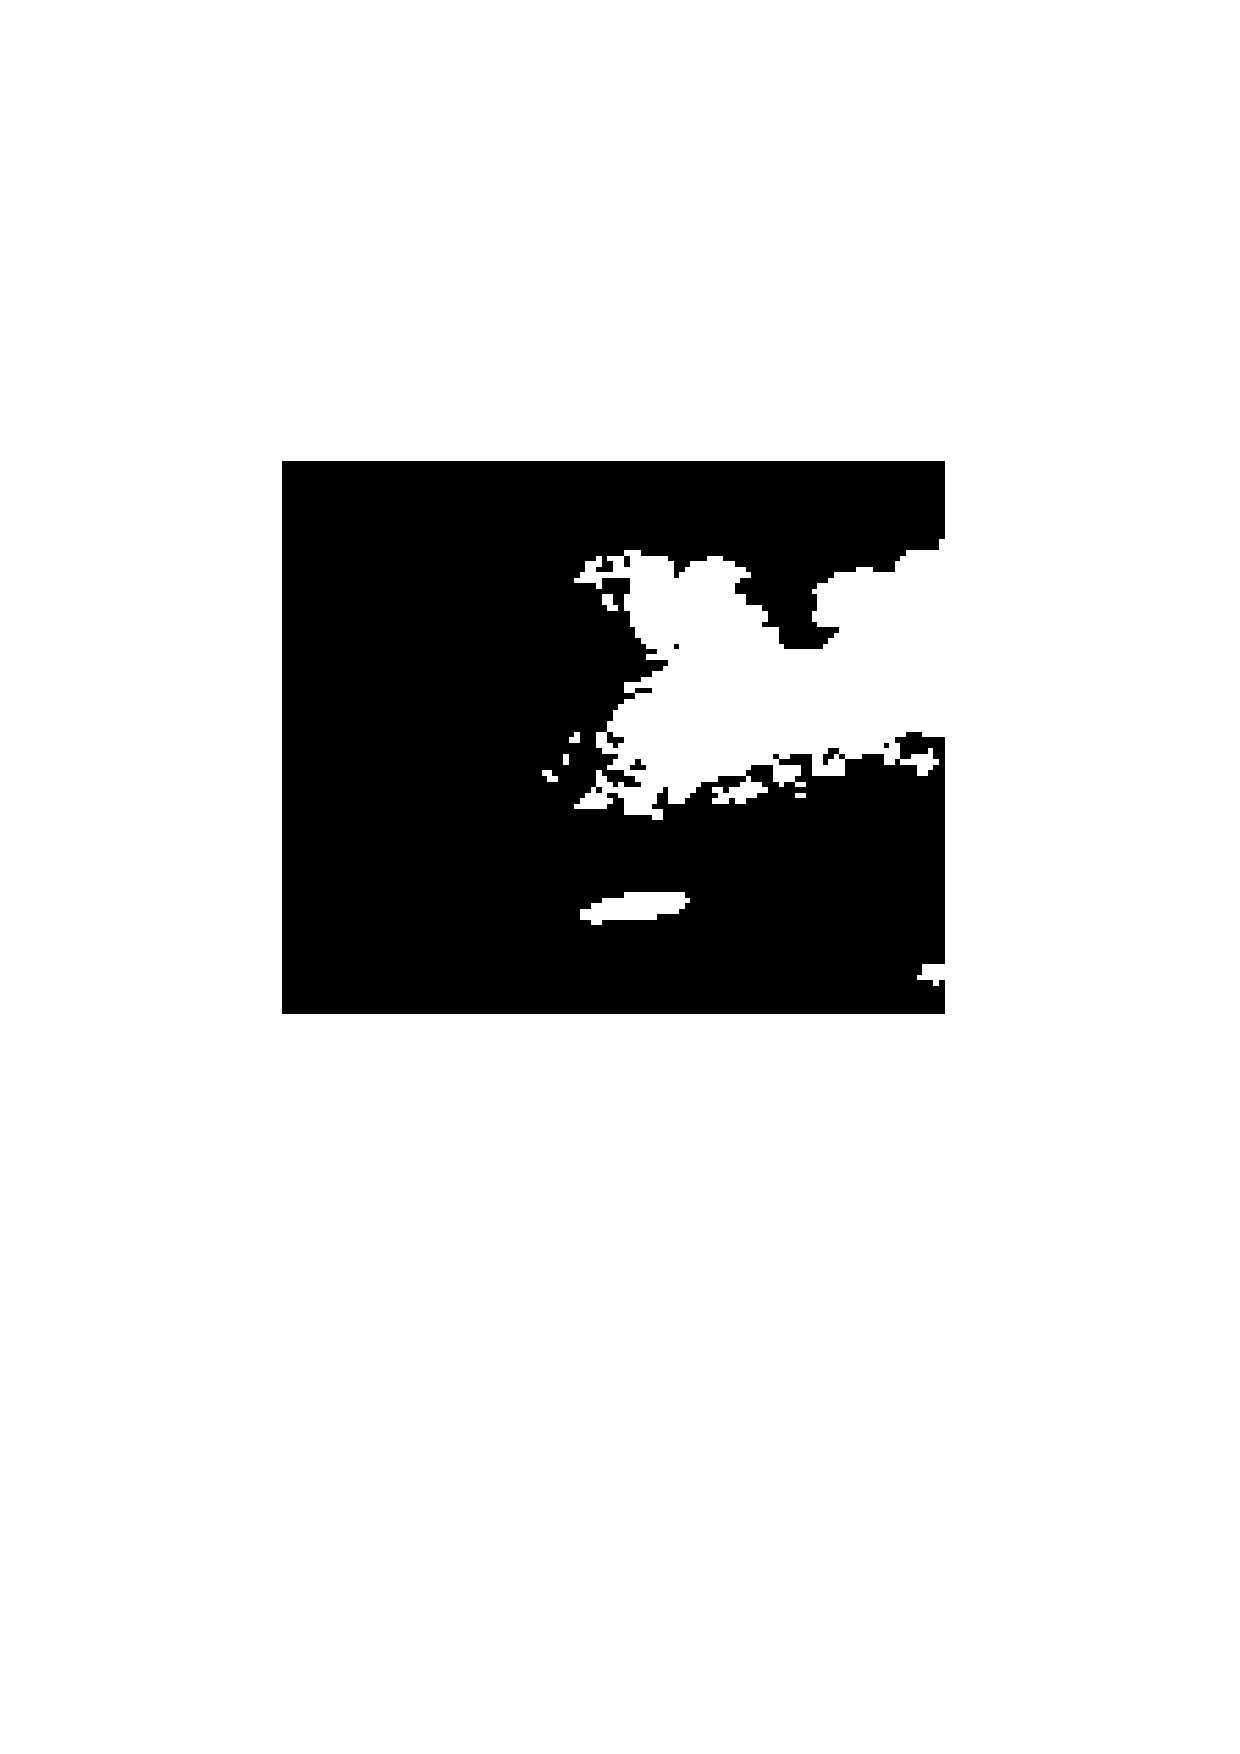
\includegraphics[height=0.25\textheight]{figures/binary}
	\caption{A binary map.}
	\label{fig:binary}
\end{figure}

\subsubsection{Baseline}
We compare the performance of our algorithms and a naive baseline of simply calculating only one main feature of the spectrum data. Usually, most differences between sea and land clutter are that the frequency for the maximum energy is almost zero. However, there are two similar peaks in sea clutter symmetrically along the zero frequency which are called Bragg peak. Thus, we can use the frequency $f$ to identify the sea/land.
\begin{equation}
f_{i, j}= \mathop{\arg\max}_{f} \ \ x(i, j, f)
\end{equation}
$x(i, j, f)$ is the energy at frequency $f_{i, j}$. As we get $f_{i, j}$, we need to compare it with the threshold $\eta$.
\[
y_{i, j}= \left\{\begin{array}{ll}
0&|f_{i, j}| > \eta, \\
1&|f_{i, j}| < \eta
\end{array}
\right.\]
0 represents the sea and 1 represents the land.
\subsection{我们的分类算法}
% A typical convolution neural network consists of a number of different layers stacked together by a deep structure: an input layer, multiple sets of convolution and pooling layers, a finite number of fully connected hidden layers, and an output layer.

典型的卷积神经网络由多个不同的层组成,它们通过深层结构堆叠在一起:输入层,多组卷积和合并层,有限数量的完全连接的隐藏层和输出层。

% The convolution layer introduces a special way of organizing a hidden element whose purpose is to take advantage of the local structure that exists in the input data. Each hidden unit is not connected to all inputs from the upper layer and is limited to only a small portion of the entire input space (for example, a small $1*3$ block). The weight of this hidden unit creates a convolution kernel, which is applied to the entire input space, resulting in feature maps. In this approach, you can reuse a set of weights for the entire input space. This is based on the premise that local useful features are also useful in other locations in the input space, which not only greatly reduces the number of parameters to be estimated, but also improves the translation invariance of the data.

卷积层引入了一种组织隐藏元素的特殊方式,其目的是利用输入数据中存在的本地结构。 每个隐藏单元不连接到上层的所有输入,并且仅限于整个输入空间的一小部分(例如,小$ 1 * 3 $块)。 该隐藏单元的权重创建一个卷积内核,该内核应用于整个输入空间,从而产生特征图。 在这种方法中,您可以为整个输入空间重用一组权重。 这是基于本地有用特征在输入空间的其他位置也是有用的前提,这不仅大大减少了要估计的参数数量,而且提高了数据的平移不变性。

Based on the actual data of our sea/land clutter spectrum and the characteristics it reflects, we construct a basic convolution neural network with six layers as shown in figure \ref{fig:struct}, each layer has multiple eigenvectors, each eigenvector has multiple neurons, and each eigenvector is derived from a feature of the convolution filter that extracts an input.
\begin{figure*}[!t]
	\centering
	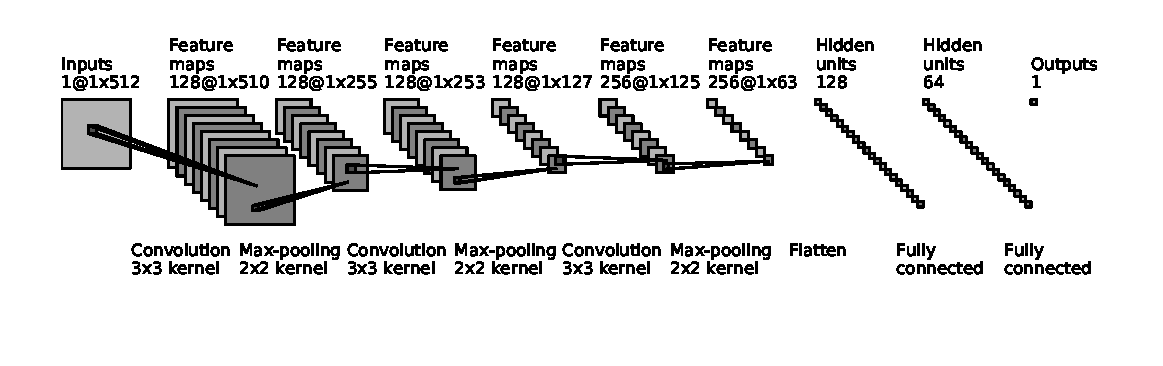
\includegraphics[width=7in]{figures/struct}
	\caption{The structure of our convolution neural network.}
	\label{fig:struct}
\end{figure*}

Step 1: Input our sea/land clutter spectral sequence (a sequence of $1 * 512$ in size) and convolve it to obtain the C1 layer. In this case, 32 neurons with a size of $1 * 3$ are used, so that each neuron in the eigenvector is connected to the $1 * 3$ neighborhood in the input, so that the feature size in the C1 layer is $1 * 510$. There are 156 trained parameters (each filter has 3 cell parameters and a bias parameter, a total of 32 filters, total $(1 * 3 + 1) * 32 = 128$ parameters), a total of $128 * (1 * 510) = 65280$ connections will be connected via the ReLU active layer.

Step 2: We apply a maximum pooling(the length is 2) process to C1 layer. The operation replaces the two adjacent features with one feature, which can help reduce the length of the feature vector, the amount of computation, and the over-fitting problem.

Step 3: After the above two steps of operation, we are equivalent to regain a new eigenvector, with this feature vector as input, repeating steps 1-2 twice, we can get a three-stage convolution neural network structure. Through the multi-stage convolution operation, the features of input vectors are fully extracted. Then, for the feature vector, flatten operation, as a convolution layer to the full connection layer of a transition, in the whole connection layer on the basis of adding dropout parameters, and then add a second layer of the whole connection, through the activation function Sigmoid. The structure of our algorithm is constructed.

Step 4: Optimize the training of our neural network model. After building a CNN model, we need to do further training on the model.

Step 5: Predictive steps. Depending on step 4, we can get the training model. In the forecasting step, we use a sliding window method to pre-process the input data. We take the same wave multi-shot window length multi-frame spectrum data averaging, as a new input to offset some interference and frequency shift.

\subsubsection{Pooling Layer}

这部分要结合实际问题讨论
% After we have acquired the features by convolution, the next step is to use these features to do the classification. In theory, people can use all the extracted features to train the classifier, such as the softmax classifier, but this is faced with the challenge of too many eigenvectors to calculate and easily leading to over-fitting.

% Because our clutter spectrum data have a static attribute, it means that the useful features in a data region are likely to be equally applicable in another region, the convolution feature can be used. Thus, in order to describe data with a large amount of data, a natural idea is to aggregate statistics for different locations, for example, one can calculate the maximum(or average) of a particular feature on an area of the sequence. These summary statistical features not only have a much lower dimension(compared to the use of all extracted features), but also improve the results(not easy to over-fitting). This aggregation is called pooling, and the commonly used pooling methods are average pooling and maximum pooling.

% These pooling units have translation invariant if the continuous range in the spectral vector is chosen as the pooled region and only the characteristics of the same (repeating) hidden cells are pooled. This means that even if the spectral vector undergoes a small translation, it will still produce the same (pooled) feature. That is, in our problem, this can be a good deal when the Bragg peaks shift.

% Formally, after obtaining the convolution features we discussed earlier, we pooled our convolution features based on the selected pooling length. We use the maximum pool, that is, select the largest value as the features of this pooling unit after the follow-up classification.

\subsubsection{Activate Function}
The choice of activation function is a very important aspect of this problem. The traditional methods usually choose Sigmod or hyperbolic tangent. However, we generally use the following ReLU activation function in the convolution neural networks.
\begin{equation}
F(x) = max (0, x)
\end{equation}
ReLU has several advantages over traditional activate function: faster calculations and more efficient gradient propagation(they are not saturated like S-shaped units), biological likelihood and sparse activation structures while still retaining sufficient discriminate nature despite their simplicity. One of its shortcomings is the initial state of the random weights, and multiple units may fall prematurely into the dead zone(a constant gradient of zero output). However, when connecting with the whole connection layer, a Sigmod activate function is better.
\begin{equation}
F(x) = \frac{1}{1-exp(x)}
\end{equation}

\subsubsection{Dropout 参数学习}
% All convolution neural network structures have a tendency to over-fit, although the number of parameters can be reduced by weight sharing. In our problems, the number of training cases is larger than an order of magnitude of evaluation cases. This may lead to the generalization beyond the scope of the sample. Therefore, we can use a simple but efficient concept, dropout, to improve the training model. In each training iteration, each concealment unit is randomly deleted with a predetermined probability, and the learning process continues normally. These random perturbations effectively prevent the network from learning fake dependencies and create complex common adaptations between hidden cells. Such a large number of neurons not only become useful in the context of other neurons. The architectural average introduced by dropout attempts to ensure that each hidden unit learning is usually conducive to generating a feature representation of the correct classification answer.
所有卷积神经网络结构都有过度拟合的趋势,尽管可以通过权重共享来减少参数的数量。 在我们的问题上,培训案例数量大于评估案件的数量级。 这可能导致超出样本范围的泛化。 因此,我们可以使用简单而有效的概念,辍学来改进培训模式。 在每次训练迭代中,以预定的概率随机删除每个隐藏单元,并且学习过程继续正常。 这些随机扰动有效地防止网络学习假依赖,并在隐藏的单元之间创建复杂的共同适应。 这样大量的神经元不仅在其他神经元的上下文中变得有用。 通过辍学引入的建筑平均值试图确保每个隐藏的单元学习通常有助于生成正确分类答案的特征表示。

\subsubsection{训练算法}
% The traditional neural network selection method is mini-batch gradient descent. The idea is to calculate the gradient of mini-batch for each iteration, and then update the parameters. However, this method has two shortcomings, one is that the choice of learning rate is difficult because of its use of the same learning rate for all parameters, the other one is that it tends to converge to a local optimum.

传统的神经网络选择方法是小批量梯度下降。 这个想法是计算每次迭代的小批量梯度,然后更新参数。 然而,这种方法有两个缺点,一个是学习率的选择是困难的,因为它对所有参数使用相同的学习率,另一个是趋向于收敛到局部最优。

% In this paper, we choose an adaptive algorithm, Adaptive Moment Estimation, which has an adaptive learning rate that dynamically adjusts the learning rate of each parameter by using the first-order moment estimation and the second-order moment estimation of the gradient. After the correction, each iterative learning rate has a clear range, making the parameters more stable.
在本文中,我们选择一种自适应算法,其具有自适应学习速率,其通过使用一阶矩估计和梯度的二阶矩估计来动态地调整每个参数的学习速率。 纠正后,每个迭代学习率都有明确的范围,使得参数更加稳定。
\subsection{数据集及分析}
我们所有的数据都是不同天数,不同地点和不同雷达配置的频谱数据。 我们查看所有频谱数据,并选择一些典型的频谱数据,如图\ref{fig:spectrum}所示。
% All the data we have are spectrum data in different days, different places and different radar configurations. We look over all the spectrum data and select some typical spectrum data as shown in figure \ref{fig:spectrum}.
%\begin{figure}[!t]
%	\centering
%	\subfloat[The spectrum for land clutters]{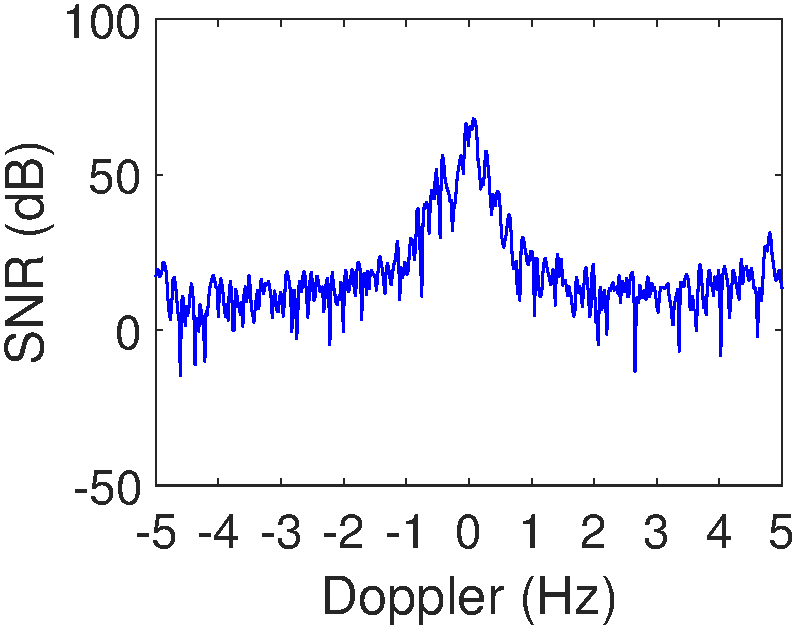
\includegraphics[width=2.5in]{figures/land}%
%		\label{fig:land}}
%	\hfil
%	\subfloat[The spectrum for sea clutters]{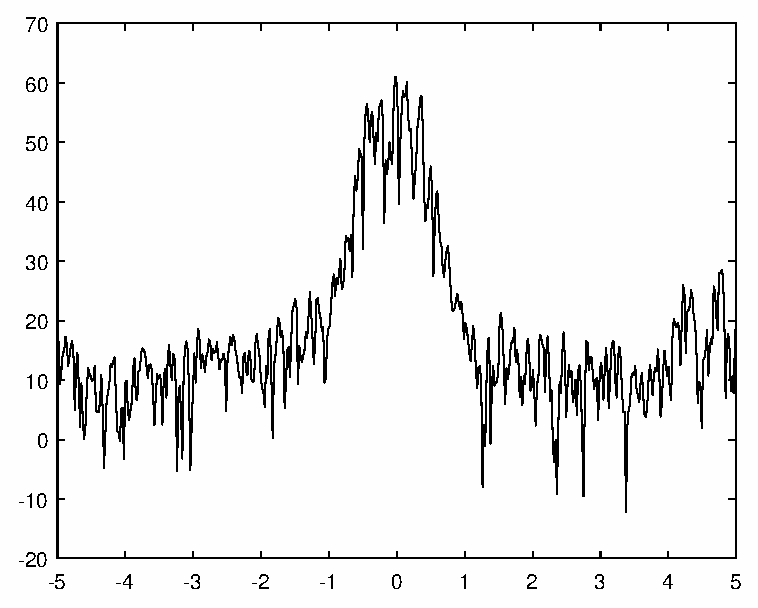
\includegraphics[width=2.5in]{figures/sea}%
%		\label{fig:sea}}
%	\caption{These two pictures are not easy to identify. \ref{fig:land} has a little shift, and the Barrage peak pf \ref{fig:sea} cannot distinguish easily.}
%	\label{fig:spectrum}
%\end{figure}

\subsubsection{数据集分组}
% In our problem, when the radar configuration changes, we may get spectrum data in a different frequency range and accuracy. For example, some data have 512 coherent accumulation points ranging from -5Hz to 5Hz and some have 256 points from -10Hz to 10Hz. Therefore, we divide all data to 4 groups:
在我们的问题中,当雷达配置发生变化时,我们可能会获得频谱数据在不同的频率范围和精度。 例如,一些数据具有从-5Hz到5Hz范围的512个相干累加点,并且一些具有从-10Hz到10Hz的256个点。 因此,我们将所有数据分为4组:

\begin{itemize}
	\item 组 A: There are 256 points from -10Hz to 10Hz shown in figure \ref{fig:case25610};
	\item Group B: There are 512 points from -5Hz to 5Hz shown in figure \ref{fig:case51205};
	\item Group C: There are 512 points from -10Hz to 10Hz shown in figure \ref{fig:case51210};
	\item Group D: There are 1024 points from -5Hz to 5Hz shown in figure \ref{fig:case102405};
\end{itemize}
% We only choose these four typical groups and give up other groups similar to them, such as data with 512 points from -10Hz to 10Hz which is similar to group B.

我们只选择这四个典型的组,放弃与他们相似的其他组,例如从-10Hz到10Hz的512点的数据,这与B组相似。

%\begin{figure*}[!t]
%	\centering
%	\subfloat[Group A]{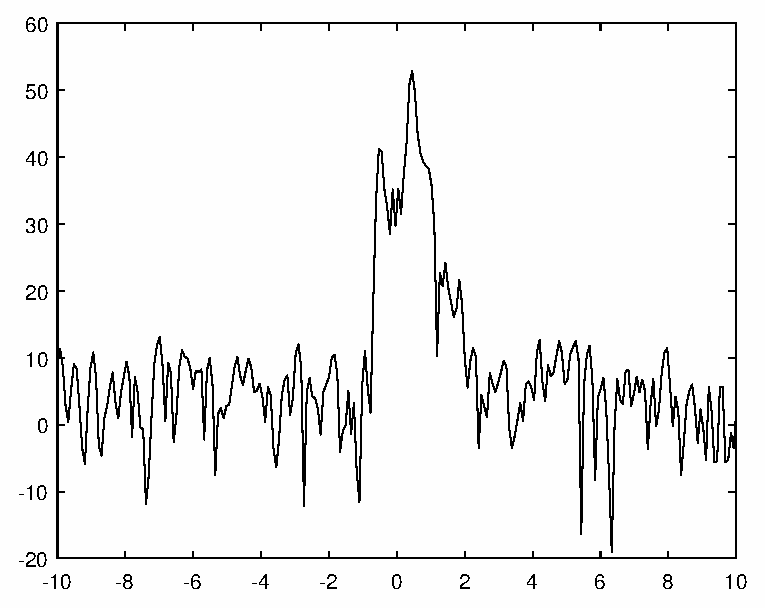
\includegraphics[width=2.5in]{figures/group256_10}%
%		\label{fig:case25610}}
%	\hfil
%	\subfloat[Group B]{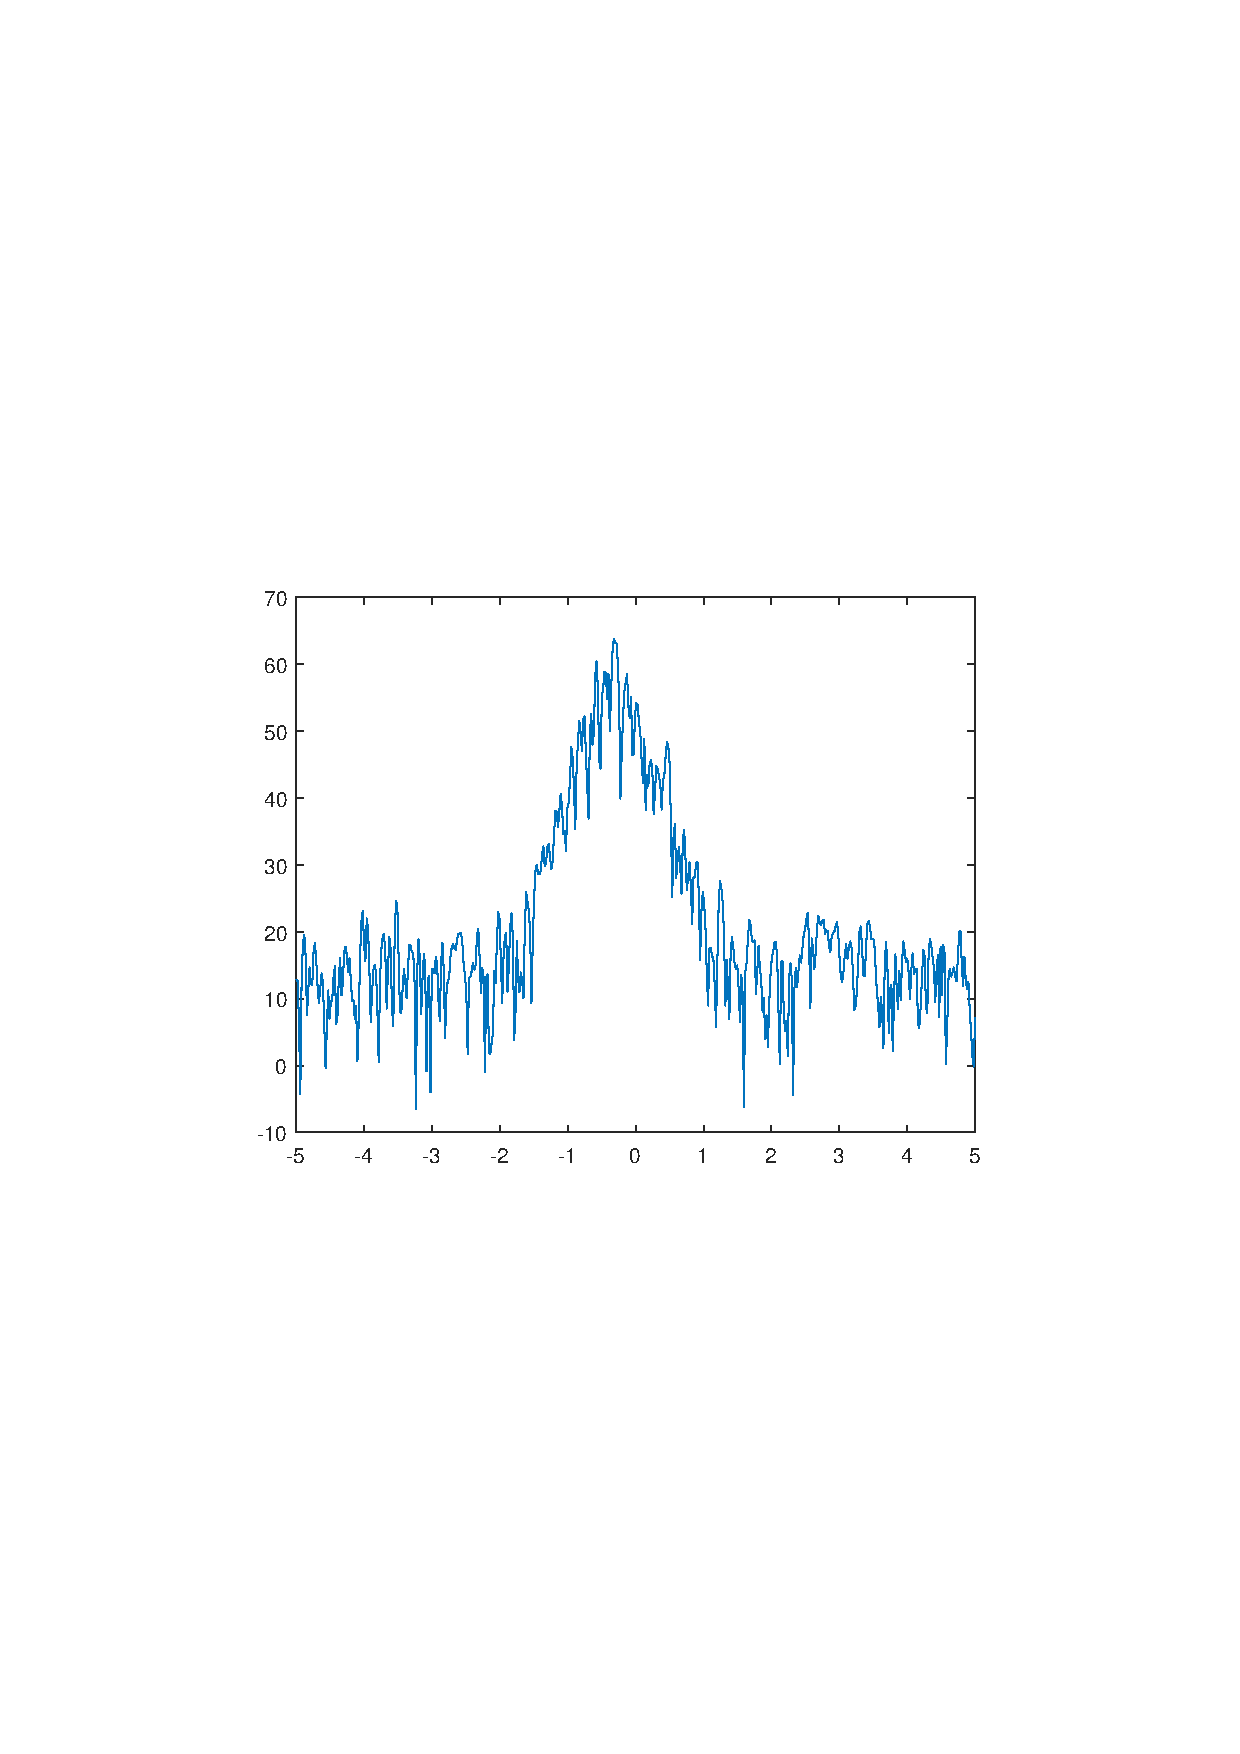
\includegraphics[width=2.5in]{figures/group512_5}%
%		\label{fig:case51205}}
%	\centering
%	\subfloat[Group C]{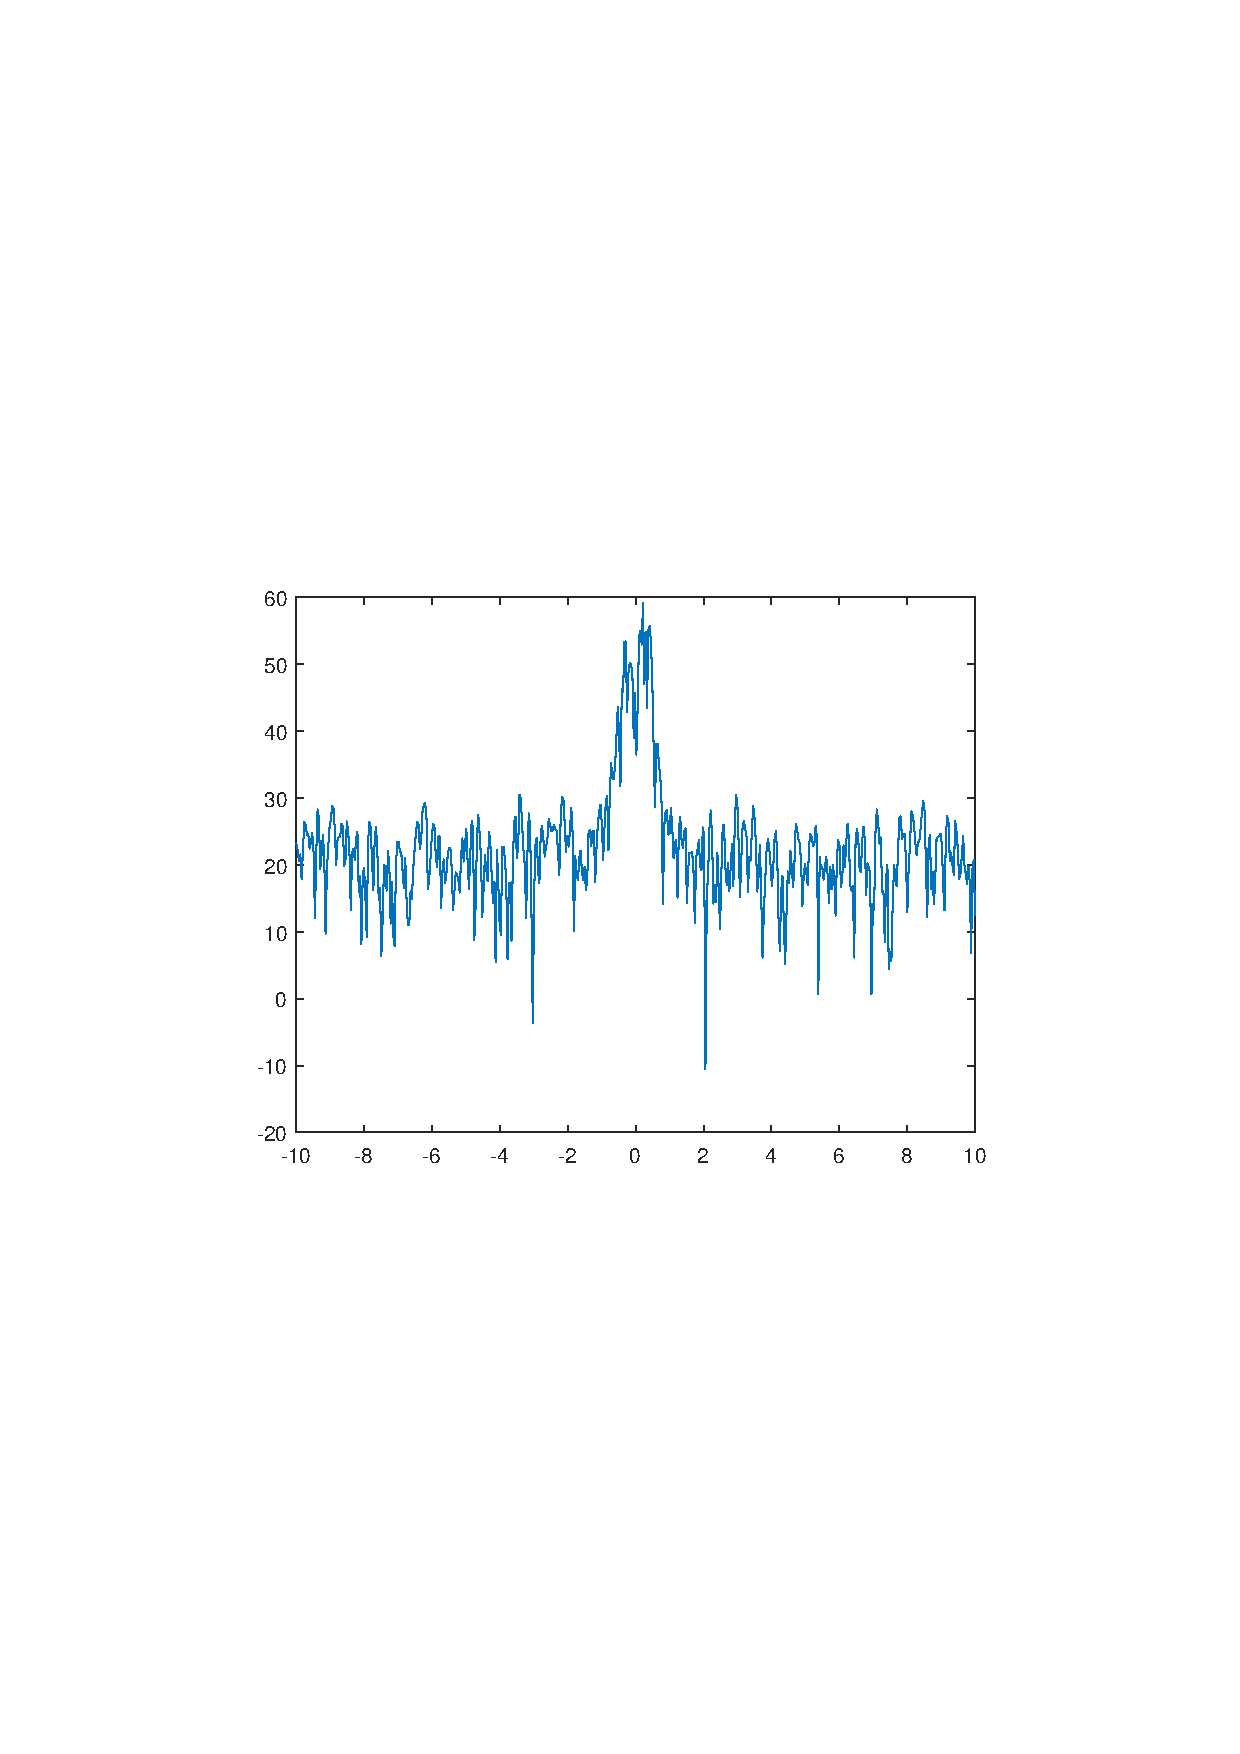
\includegraphics[width=2.5in]{figures/group512_10}%
%		\label{fig:case51210}}
%	\hfil
%	\subfloat[Group D]{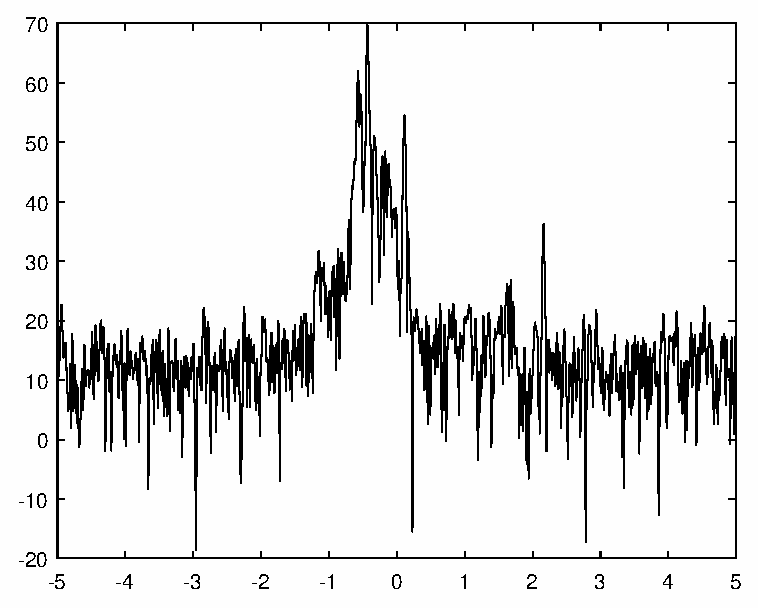
\includegraphics[width=2.5in]{figures/group1024_5}%
%		\label{fig:case102405}}
%	\caption{Different group spectrum data.}
%	\label{fig:group}
%\end{figure*}



\section{地海杂波分类评估}
在本节中,我们评估以前提供的模型的性能。
% In this section, we evaluate the performance of the model presented before.
\subsection{算法实现}
% We compare our algorithms with two other algorithms, traditional single feature recognition algorithms and SVM algorithms. Three characteristics of sea/land clutter selected for SVM are:
我们比较我们的算法与另外两种算法,传统的单特征识别算法和SVM算法。 选择SVM的海/陆杂波的三个特征是:
\begin{itemize}
	\item 最大后向散射幅值
	\item 频谱中最大与次大幅值频率之差
	\item 频谱中最大与次大幅值幅度之差
\end{itemize}
% To ensure that we have enough data to train and test our algorithm, we consider several frame data(there are about 20000 spectrum data for every frame) in different conditions. We also randomly select $70\%$ of data as training data, 10 percent is used as validation data and others are test data. As described before, the area ratio is used for evaluate the data near the border of sea and land.
为了确保我们有足够的数据来训练和测试我们的算法,我们在不同的条件下考虑几个帧数据(每帧约有20000个频谱数据)。 我们还随机选择$ 70 \%$的数据作为培训数据,$ 10 \%$用作交叉验证数据,其他数据用作测试数据。 如前所述,面积比用于评估海陆边界附近的数据。

\subsection{Overall Quality}

% In order to test the universality of our algorithm, we test our method, SVM and the baseline algorithm in four groups dataset as described preceding section shown in figure \ref{fig:group_results}. Figure \ref{fig:group_results} shows our algorithm can have a good results in different dataset groups. Although, for the same neural network structure, the first dataset group converges in the largest epoch times. This is because that there is less information or features when the ratio of frequency and points goes smaller.
为了测试我们的算法的普遍性,我们在四组数据集中测试我们的方法,SVM和基线算法,如上图所示,如图\ref{fig:group_results}所示。 图\ref{fig:group_results}显示我们的算法可以在不同的数据集组中获得良好的结果。 虽然,对于相同的神经网络结构,第一个数据集群收敛于最大的时代。 这是因为当频率和点的比例变小时信息或特征较少。
\begin{figure}[!t]
	\centering
	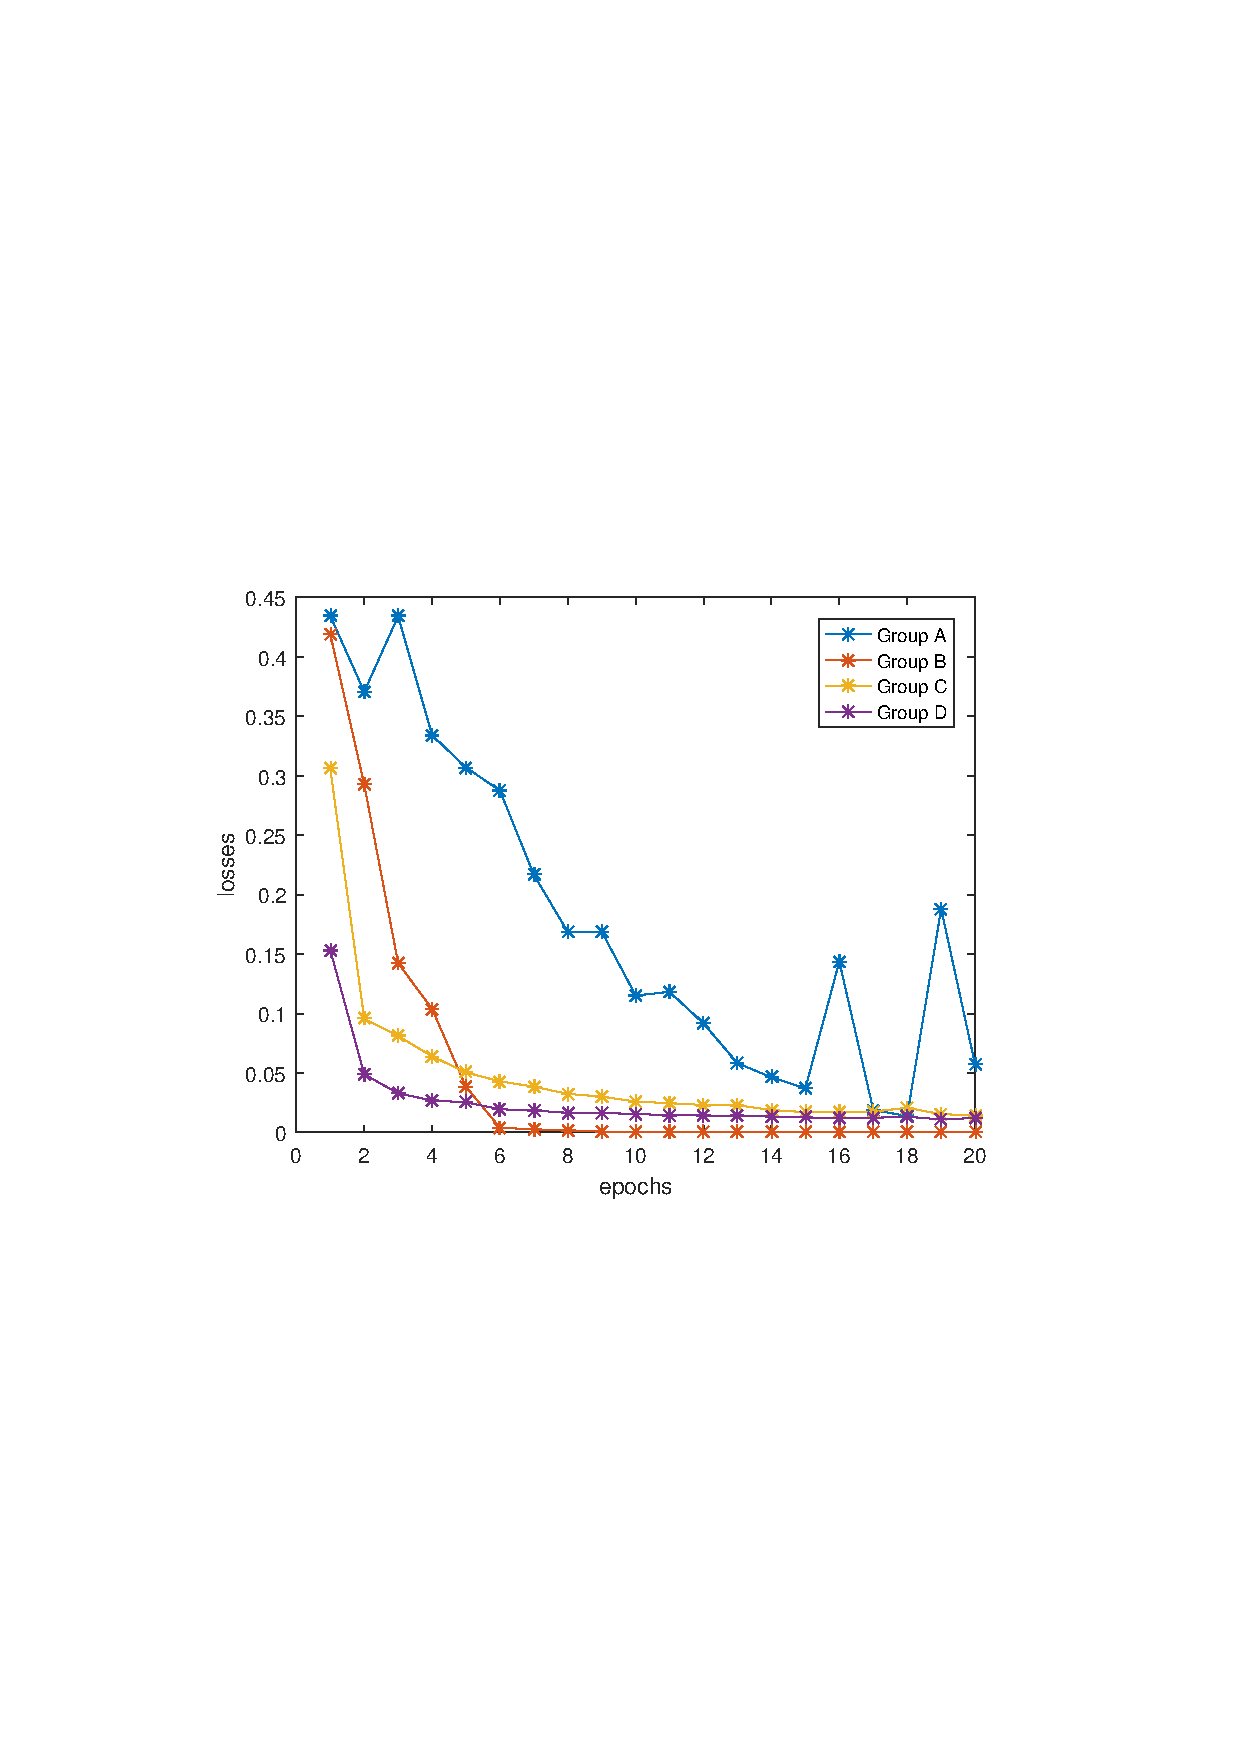
\includegraphics[width=3.5in]{figures/group_results}
	\caption{The losses for different dataset groups.}
	\label{fig:group_results}
\end{figure}

% As we described before, there are another two usual methods to solve our problem. We did some experiments to combine our algorithm with them. Table \ref{tab:methods} shows the correct rate and matching rate. Our method meets the best result in both experiments. Besides, when finding the largest matching rate through the whole world map, the mating rates for the three methods to their paired maps in some time seem to differ a little. However, we can find that both SVM and baseline method pair to wrong zones.
正如我们之前描述的,还有另外两种常用的方法来解决我们的问题。 我们做了一些实验来结合我们的算法与他们。 表\ref{tab:methods}显示正确的速率和匹配率。 我们的方法在两个实验中都达到最佳效果。 此外,当通过整个世界地图找到最大的匹配率时,三种方法与其配对地图在一段时间内的交配率似乎有所不同。 然而,我们可以发现SVM和基线方法都对错了区域。
\begin{table}[!t]
	\renewcommand{\arraystretch}{1.3}
	\caption{Correct and matching rate comparing of three methods.}
	\label{tab:methods}
	\centering
	\begin{tabular}{c|ccc}
		\hline
		& Our method & SVM & Baseline \\
		\hline
		Correct Rate & 99.69\% & 92.44\% & 81.85\% \\
		\hline
		Largest Matching Rate & 88.99\% & 22.77\% & 23.48\% \\
		\hline
		Matching Rate & 88.99\% & 81.31\% & 88.21\% \\
		\hline
	\end{tabular}
\end{table}

% Figure \ref{fig:sizes} shows the average classification accuracy rate for different sample sizes. As the baseline method only uses a threshold got according to prior knowledge, it differs a little as the dataset grows. Our learning method has a better result as the data volume increases.
图\ref{fig:sizes}显示不同样本大小的平均分类准确率。 由于基线方法仅使用根据先验知识得到的阈值,因此随数据集增长而变化不大。 随着数据量的增加,我们的学习方法有了更好的效果。
\begin{figure}[!t]
	\centering
	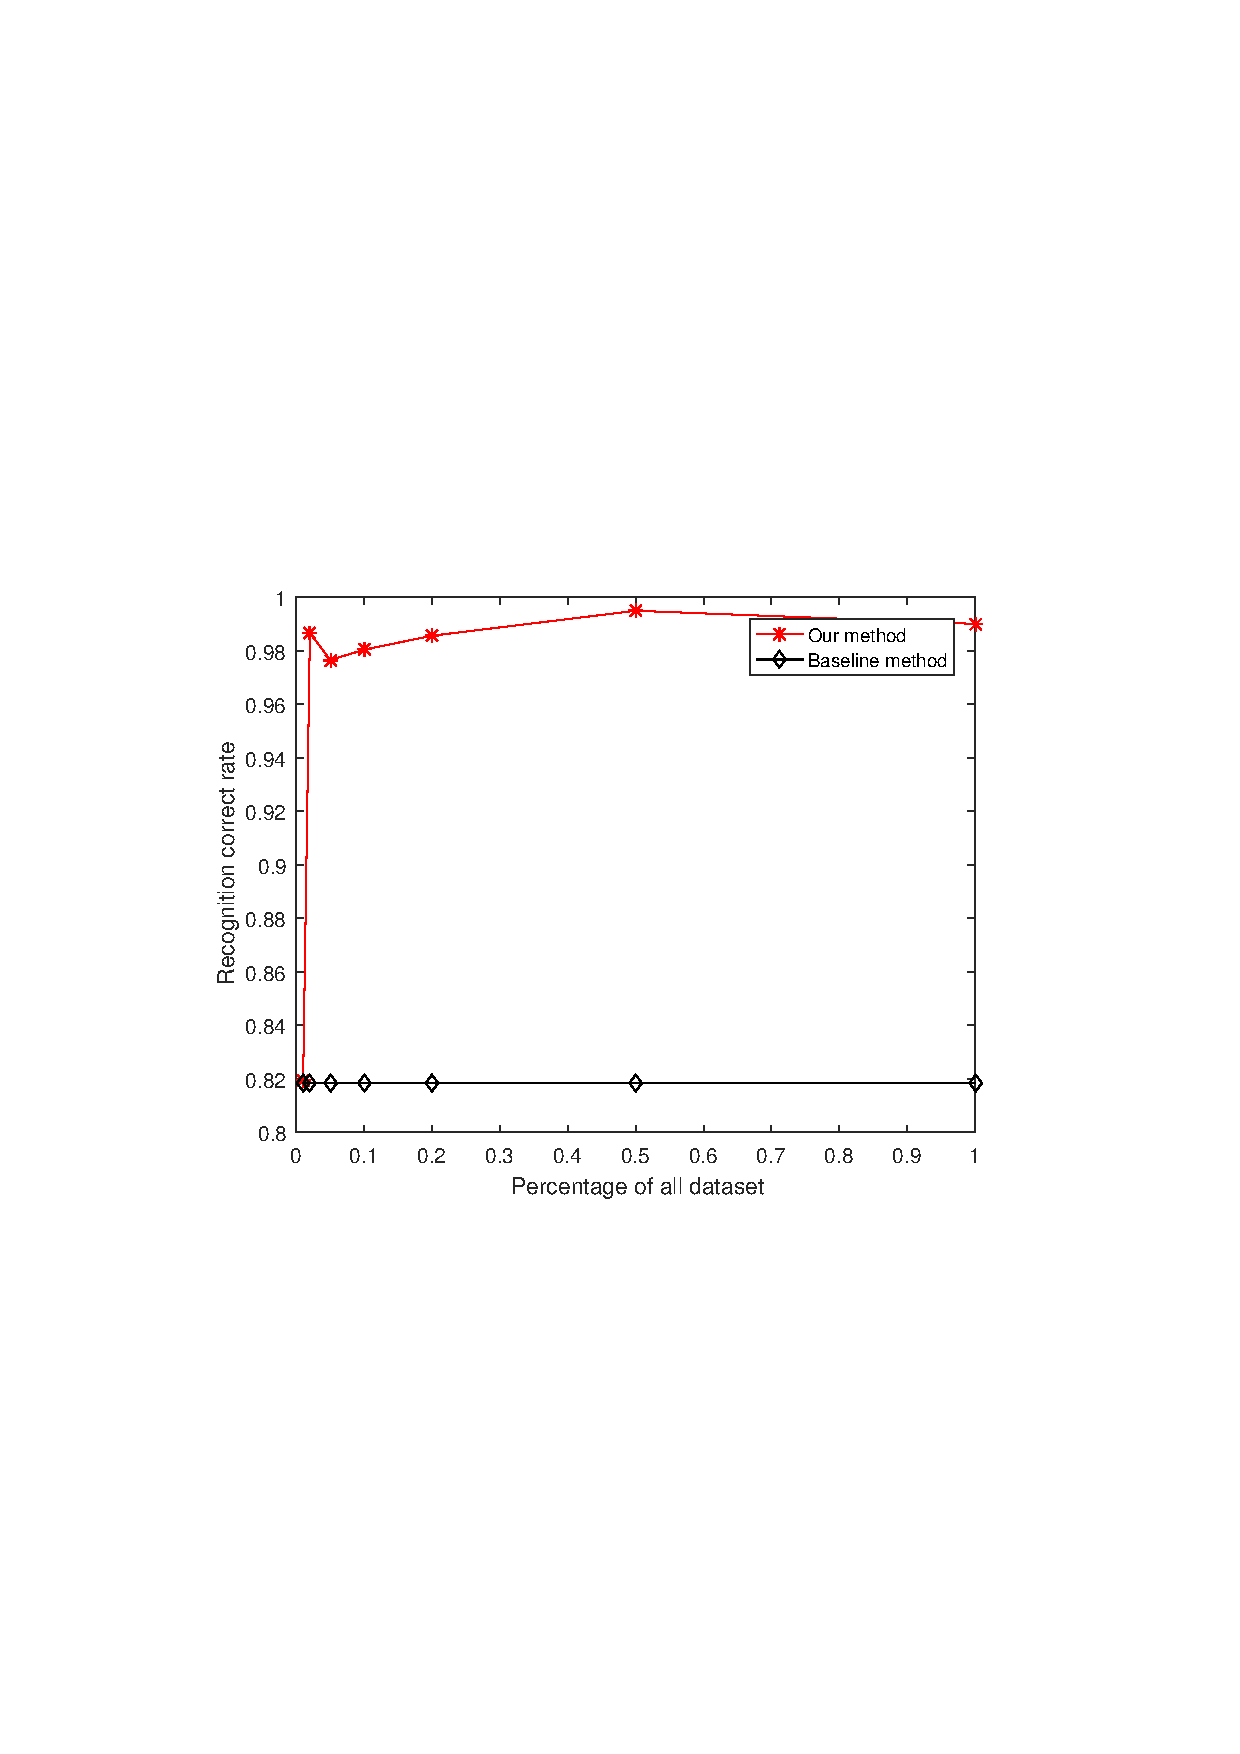
\includegraphics[width=3.5in]{figures/sizes}
	\caption{The experiments of comparing our method and baseline method against sample sizes of dataset.}
	\label{fig:sizes}
\end{figure}
% As we all know that parameters of convolution neural network play an important role in classification correct rate. Therefore, we first do some experiments to show the accuracy of validation data when epoch and batch differs. In fig \ref{fig:epoch}, we can easily see that the accuracy grows along with increasing of epoch times. Besides, larger is the batch, easier it is to converge.
众所周知,卷积神经网络的参数在分类正确率中起着重要的作用。 因此,我们首先做一些实验来显示时代和批次不同的验证数据的准确性。 在图\ref{fig:epoch}中,我们可以很容易地看出,准确度随着时代的增加而增长。 此外,批量更大,收敛更容易。
\begin{figure}[!t]
	\centering
	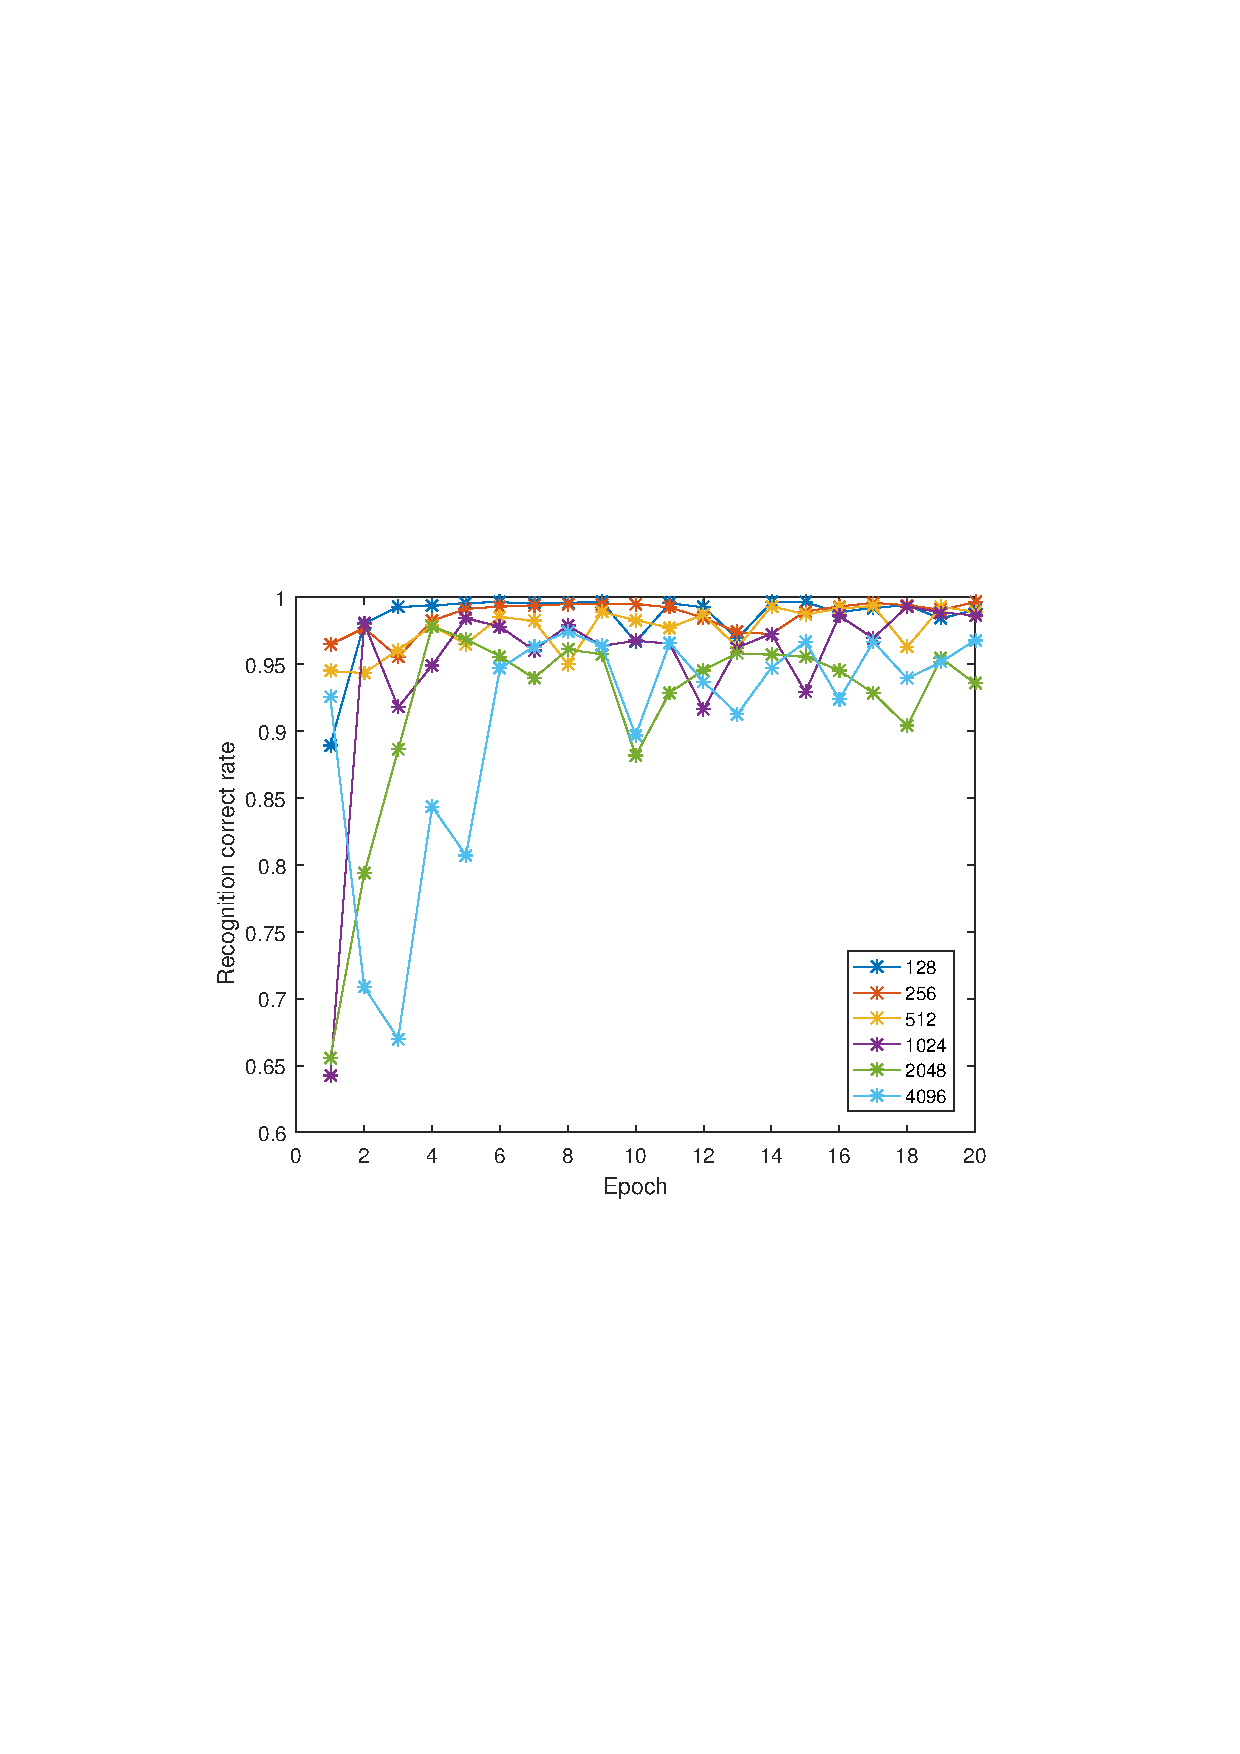
\includegraphics[width=3.5in]{figures/epoch}
	\caption{Validation accuracy against epochs for different batches.}
	\label{fig:epoch}
\end{figure}

融合预处理参数设计由于滑窗算法的很重要的一个参数就是窗长,针对于本问题主要考虑到电离层会发生变化,过长的窗长对无法及时的响应电离层的变化,影响识别准确率以及地图匹配精度。为了取得一个合适的窗长,我们首先利用不同窗长平均融合后的数据进行测试,得到图 20的结果,该结果也证明了在窗长过长时候,准确率会下降的结论,当窗长过大时准确率会降到比窗长为1时还要低。 图 23 不同窗长识别结果对比图为了进一步比较权重的变化对于识别结果的影响,我们设窗长为 ,样本 的权重为 ,则有融合后的样本为 ,当取权重为 时,得到下面结果,故根据实验结果,本课题最终选择窗长长度为3 图 24 更改权重后不同窗长识别结果对比4.2目标定位精度修正验证由于缺乏实际的 变换相关的航迹信息,故无法对定位精度修正系数进行一个很好的验证。这里我们采用地图变换的过程来进行辅助验证。其基本流程与目标的定位精度修正类似。首先将整个匹配地图划分为很多小的匹配区域,然后对于每个匹配区域分别进行修正系数计算。

As we described before, we use a fusion method to avoid the saltation change in spectrum sequence. Figure \ref{fig:window} shows that the matching rate grows as the window length increases at first, and then it decreases.
\begin{figure}[!t]
	\centering
	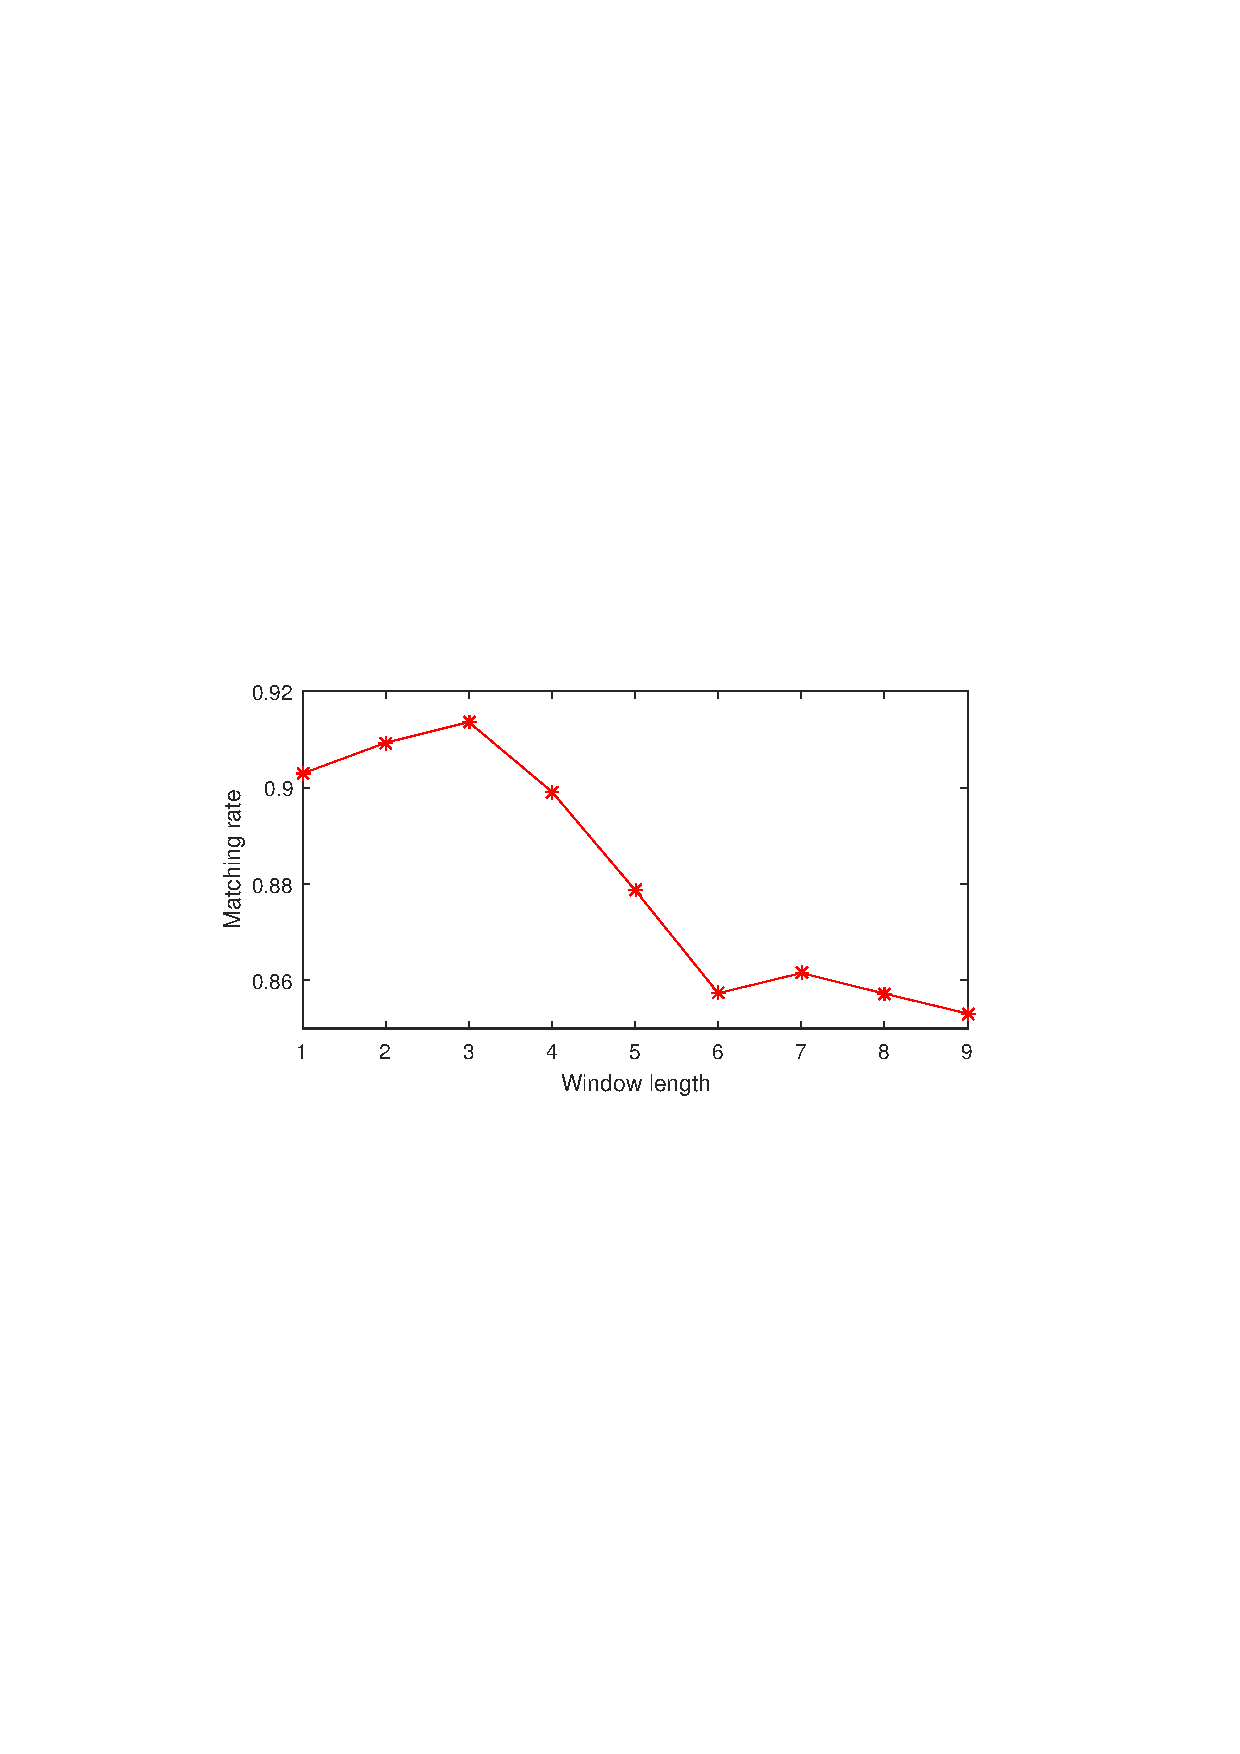
\includegraphics[width=3.5in]{figures/window}
	\caption{The matching rate against fusion window length.}
	\label{fig:window}
\end{figure}
为了找出区分海洋/陆地结果的最佳阈值,我们使用不同的概率阈值计算相同测试数据的正确率。 图\ref{fig:threshold}显示,随着阈值越大,增长速度越慢,速率越快。 另一方面,当阈值仅为$0.01$时,识别率仍高于$0.86$。 识别我们的方法的概率大多令人信服,如\ref{fig:prob}所示。
% To find the best threshold to distinguish sea/land result, we calculate the correct rate of the same test data using different probability threshold. Figure \ref{fig:threshold} shows that rate increases as the threshold is larger and the growth rate becomes slower. In the other aspect, when the threshold is only $0.01$, the recognition rate is still higher than $0.86$. The probabilities of recognition our method are mostly convincing as shown in \ref{fig:prob}.
\begin{figure}[!t]
	\centering
	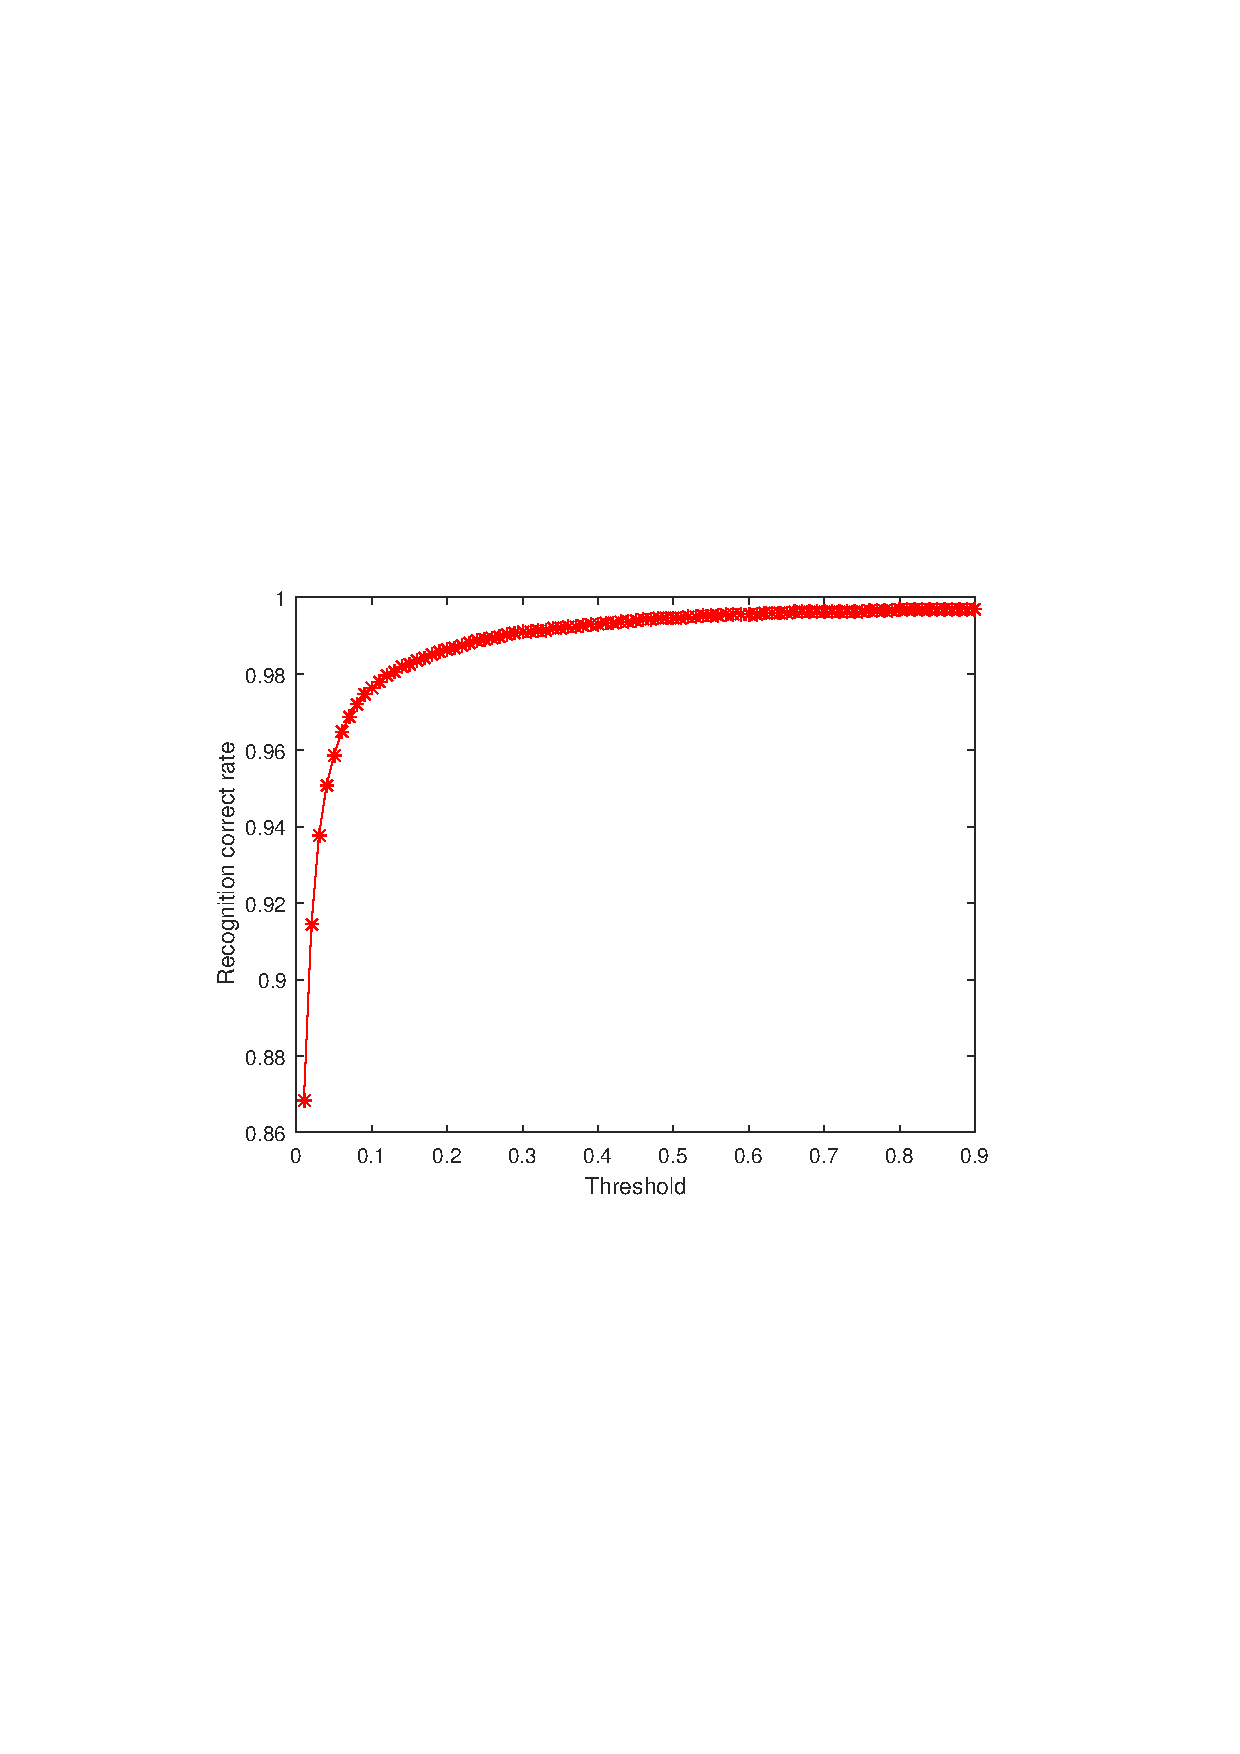
\includegraphics[width=3.5in]{figures/threashold}
	\caption{The recognition correct rate against the threshold.}
	\label{fig:threshold}
\end{figure}
\begin{figure}[!t]
	\centering
	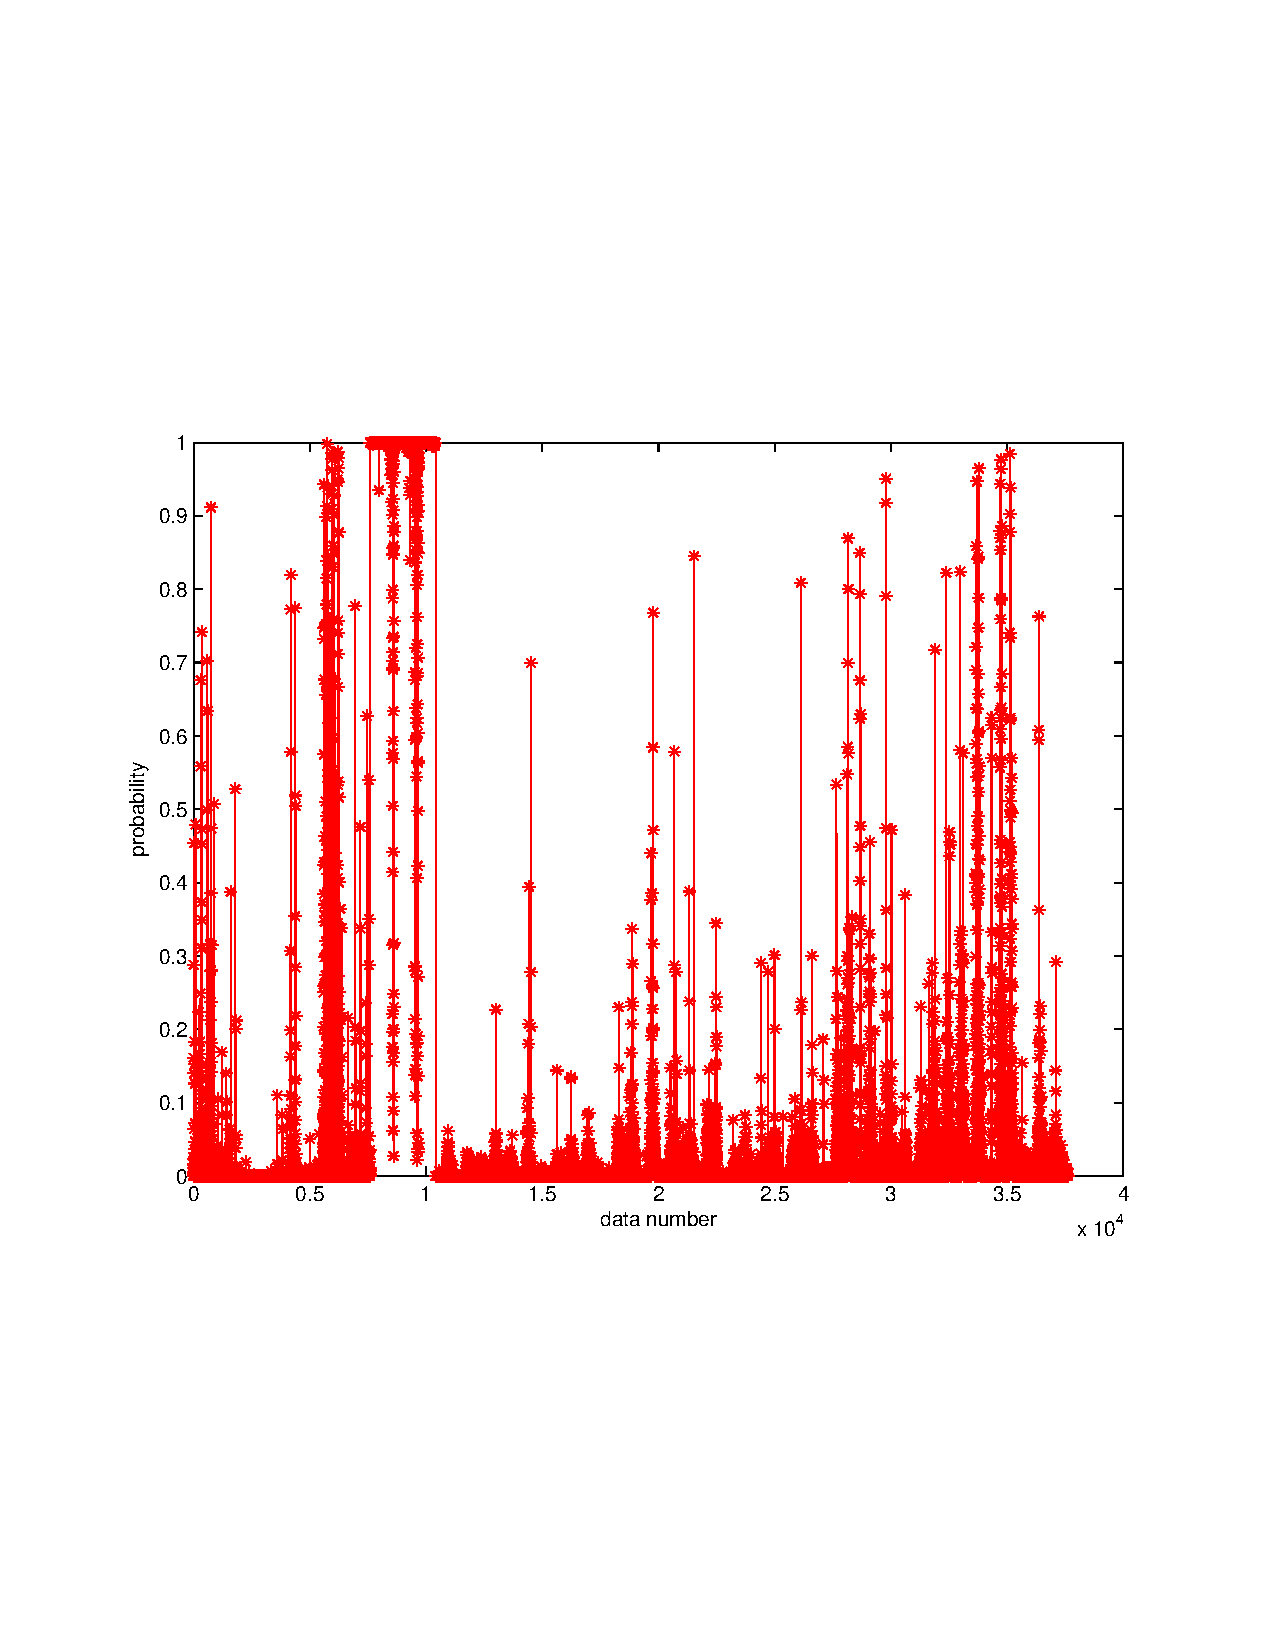
\includegraphics[width=3.5in]{figures/prob}
	\caption{The recognition correct rate against the data number.}
	\label{fig:prob}
\end{figure}
%\begin{itemize}
%	\item different window and no window
%	\item figures of loss function with time
%	\item dropout changes
%	\item probability threshold changes
%
%	\item fusion and not fusion
%\end{itemize}
\subsection{Feature Visualization}
% todo feature visulation

识别结果的理论分析上面利用大量的测试数据的识别结果以及地图匹配结果对于算法进行了验证,这里我们通过理论分析,验证了算法的合理性。通过计算当输入数据的某个数据点发生变化时输出梯度的变化,得到每一个数据点对于输出梯度的影响,从而得到该频谱数据关注度图。下图红色圆圈部分表示主要利用的特征所在多普勒频率,可以很直观地看出,对于下图这样的海杂波布拉格峰附件频点的数据被关注比较多,另一方面同时兼顾了其余频点的特征,提高了识别准确率。 图 22 某距离方位单元海杂波频谱数据关注度图

There is a problem for the CNN method is that we cannot estimate the feature we learn intuitively. Therefore, in this section, we use a gradient-based visualization method to show the support feature for the result using our trained model. We define a sequence of our spectrum data as$ S = \{s_1, s_2, .., s_n\} $, where $n$ is the number of points in the sequence, and our output probability $p(S)$. Thus, we can get:
\begin{equation}
p(S) = w^TS+b,
\end{equation}
where $w$ and $b$ are respectively the weight and bias of our model. In fact, the weight $w$ here shows the importance of corresponding points. In our model, the class probability function $p(S)$ is a highly non-linear function, a Taylor method is used here to approximate $p(S)$. To simplify the calculation, we use first-order Taylor expansion:
\begin{equation}
w = \frac{\partial{p}}{\partial{S}}{\mid}_{s_i}
\label{equ:w}
\end{equation}
Therefore, we can get the $w$ in equation \ref{equ:w} can be calculated by back-propagation, which is not needed to describe clearly. Figure \ref{fig:vis} shows that the features mainly focus on the data as we have expected.
\begin{figure}[!t]
	\centering
%	\includefigures[width=3.5in]{figures/heatmap}
	\caption{The heat map for features that play import roles.}
	\label{fig:vis}
\end{figure}
\section{小结}
% In this paper, the sea/land clutter identification problem of OTHR target localization accuracy is proposed in a novel algorithm based on convolution neural network. The traditional threshold recognition method or SVM algorithm extracts the features from spectrum data according to the experience, which leads to the operation complexity and the low classification precision. The CNN-based sea/land recognition method does not have the above shortcomings.
在本文中,基于卷积神经网络的新算法提出了OTHR目标定位精度的海/陆杂波识别问题。 传统的阈值识别方法或SVM算法根据经验从频谱数据中提取特征,导致操作复杂度高,分类精度低。 基于CNN的海陆识别方法没有上述缺点。
% In this paper, our algorithm is compared with the traditional algorithm and SVM algorithm. The experiments show that our method is efficient and reliable in the sea/land identification problem. With the help of the classification results, we can get a precise correction factor for our target tracking problem.
在本文中,我们的算法与传统算法和SVM算法进行了比较。 实验表明,我们的方法在海域/陆地识别问题上有效可靠。 在分类结果的帮助下,我们可以得到我们的目标跟踪问题的精确校正因子。
